\documentclass[twoside]{book}

% Packages required by doxygen
\usepackage{calc}
\usepackage{doxygen}
\usepackage{graphicx}
\usepackage[utf8]{inputenc}
\usepackage{makeidx}
\usepackage{multicol}
\usepackage{multirow}
\usepackage{textcomp}
\usepackage[table]{xcolor}

% Font selection
\usepackage[T1]{fontenc}
\usepackage{mathptmx}
\usepackage[scaled=.90]{helvet}
\usepackage{courier}
\usepackage{amssymb}
\usepackage{sectsty}
\renewcommand{\familydefault}{\sfdefault}
\allsectionsfont{%
  \fontseries{bc}\selectfont%
  \color{darkgray}%
}
\renewcommand{\DoxyLabelFont}{%
  \fontseries{bc}\selectfont%
  \color{darkgray}%
}

% Page & text layout
\usepackage{geometry}
\geometry{%
  a4paper,%
  top=2.5cm,%
  bottom=2.5cm,%
  left=2.5cm,%
  right=2.5cm%
}
\tolerance=750
\hfuzz=15pt
\hbadness=750
\setlength{\emergencystretch}{15pt}
\setlength{\parindent}{0cm}
\setlength{\parskip}{0.2cm}
\makeatletter
\renewcommand{\paragraph}{%
  \@startsection{paragraph}{4}{0ex}{-1.0ex}{1.0ex}{%
    \normalfont\normalsize\bfseries\SS@parafont%
  }%
}
\renewcommand{\subparagraph}{%
  \@startsection{subparagraph}{5}{0ex}{-1.0ex}{1.0ex}{%
    \normalfont\normalsize\bfseries\SS@subparafont%
  }%
}
\makeatother

% Headers & footers
\usepackage{fancyhdr}
\pagestyle{fancyplain}
\fancyhead[LE]{\fancyplain{}{\bfseries\thepage}}
\fancyhead[CE]{\fancyplain{}{}}
\fancyhead[RE]{\fancyplain{}{\bfseries\leftmark}}
\fancyhead[LO]{\fancyplain{}{\bfseries\rightmark}}
\fancyhead[CO]{\fancyplain{}{}}
\fancyhead[RO]{\fancyplain{}{\bfseries\thepage}}
\fancyfoot[LE]{\fancyplain{}{}}
\fancyfoot[CE]{\fancyplain{}{}}
\fancyfoot[RE]{\fancyplain{}{\bfseries\scriptsize Generated on Wed Jun 24 2015 19\-:12\-:20 for Mensajer\-O/\-Server by Doxygen }}
\fancyfoot[LO]{\fancyplain{}{\bfseries\scriptsize Generated on Wed Jun 24 2015 19\-:12\-:20 for Mensajer\-O/\-Server by Doxygen }}
\fancyfoot[CO]{\fancyplain{}{}}
\fancyfoot[RO]{\fancyplain{}{}}
\renewcommand{\footrulewidth}{0.4pt}
\renewcommand{\chaptermark}[1]{%
  \markboth{#1}{}%
}
\renewcommand{\sectionmark}[1]{%
  \markright{\thesection\ #1}%
}

% Indices & bibliography
\usepackage{natbib}
\usepackage[titles]{tocloft}
\setcounter{tocdepth}{3}
\setcounter{secnumdepth}{5}
\makeindex

% Hyperlinks (required, but should be loaded last)
\usepackage{ifpdf}
\ifpdf
  \usepackage[pdftex,pagebackref=true]{hyperref}
\else
  \usepackage[ps2pdf,pagebackref=true]{hyperref}
\fi
\hypersetup{%
  colorlinks=true,%
  linkcolor=blue,%
  citecolor=blue,%
  unicode%
}

% Custom commands
\newcommand{\clearemptydoublepage}{%
  \newpage{\pagestyle{empty}\cleardoublepage}%
}


%===== C O N T E N T S =====

\begin{document}

% Titlepage & ToC
\hypersetup{pageanchor=false}
\pagenumbering{roman}
\begin{titlepage}
\vspace*{7cm}
\begin{center}%
{\Large Mensajer\-O/\-Server \\[1ex]\large 1.\-0.\-0 }\\
\vspace*{1cm}
{\large Generated by Doxygen 1.8.6}\\
\vspace*{0.5cm}
{\small Wed Jun 24 2015 19:12:20}\\
\end{center}
\end{titlepage}
\clearemptydoublepage
\tableofcontents
\clearemptydoublepage
\pagenumbering{arabic}
\hypersetup{pageanchor=true}

%--- Begin generated contents ---
\chapter{Hierarchical Index}
\section{Class Hierarchy}
This inheritance list is sorted roughly, but not completely, alphabetically\-:\begin{DoxyCompactList}
\item \contentsline{section}{Clock}{\pageref{classClock}}{}
\item \contentsline{section}{Constants}{\pageref{classConstants}}{}
\item \contentsline{section}{Conversation}{\pageref{classConversation}}{}
\item \contentsline{section}{Database}{\pageref{classDatabase}}{}
\item \contentsline{section}{Event\-Handler}{\pageref{classEventHandler}}{}
\begin{DoxyCompactList}
\item \contentsline{section}{S\-I\-G\-I\-N\-T\-\_\-\-Handler}{\pageref{classSIGINT__Handler}}{}
\end{DoxyCompactList}
\item \contentsline{section}{Loggero}{\pageref{classLoggero}}{}
\item \contentsline{section}{Message}{\pageref{classMessage}}{}
\item \contentsline{section}{Message\-Factory}{\pageref{classMessageFactory}}{}
\item \contentsline{section}{Proceso}{\pageref{classProceso}}{}
\begin{DoxyCompactList}
\item \contentsline{section}{Server}{\pageref{classServer}}{}
\end{DoxyCompactList}
\item \contentsline{section}{Service\-Layer}{\pageref{classServiceLayer}}{}
\item \contentsline{section}{Signal\-Handler}{\pageref{classSignalHandler}}{}
\item \contentsline{section}{User}{\pageref{classUser}}{}
\item \contentsline{section}{User\-Factory}{\pageref{classUserFactory}}{}
\end{DoxyCompactList}

\chapter{Class Index}
\section{Class List}
Here are the classes, structs, unions and interfaces with brief descriptions\-:\begin{DoxyCompactList}
\item\contentsline{section}{\hyperlink{classClock}{Clock} }{\pageref{classClock}}{}
\item\contentsline{section}{\hyperlink{classConstants}{Constants} }{\pageref{classConstants}}{}
\item\contentsline{section}{\hyperlink{classConversation}{Conversation} }{\pageref{classConversation}}{}
\item\contentsline{section}{\hyperlink{classDatabase}{Database} }{\pageref{classDatabase}}{}
\item\contentsline{section}{\hyperlink{classEventHandler}{Event\-Handler} }{\pageref{classEventHandler}}{}
\item\contentsline{section}{\hyperlink{classLoggero}{Loggero} }{\pageref{classLoggero}}{}
\item\contentsline{section}{\hyperlink{classMessage}{Message} }{\pageref{classMessage}}{}
\item\contentsline{section}{\hyperlink{classMessageFactory}{Message\-Factory} }{\pageref{classMessageFactory}}{}
\item\contentsline{section}{\hyperlink{classProceso}{Proceso} }{\pageref{classProceso}}{}
\item\contentsline{section}{\hyperlink{classServer}{Server} }{\pageref{classServer}}{}
\item\contentsline{section}{\hyperlink{classServiceLayer}{Service\-Layer} }{\pageref{classServiceLayer}}{}
\item\contentsline{section}{\hyperlink{classSIGINT__Handler}{S\-I\-G\-I\-N\-T\-\_\-\-Handler} }{\pageref{classSIGINT__Handler}}{}
\item\contentsline{section}{\hyperlink{classSignalHandler}{Signal\-Handler} }{\pageref{classSignalHandler}}{}
\item\contentsline{section}{\hyperlink{classUser}{User} }{\pageref{classUser}}{}
\item\contentsline{section}{\hyperlink{classUserFactory}{User\-Factory} }{\pageref{classUserFactory}}{}
\end{DoxyCompactList}

\chapter{Class Documentation}
\hypertarget{classClock}{\section{Clock Class Reference}
\label{classClock}\index{Clock@{Clock}}
}
\subsection*{Static Public Member Functions}
\begin{DoxyCompactItemize}
\item 
static string \hyperlink{classClock_ae5650d533bb7af21255d5e0031b89bf2}{get\-Time} ()
\end{DoxyCompactItemize}


\subsection{Member Function Documentation}
\hypertarget{classClock_ae5650d533bb7af21255d5e0031b89bf2}{\index{Clock@{Clock}!get\-Time@{get\-Time}}
\index{get\-Time@{get\-Time}!Clock@{Clock}}
\subsubsection[{get\-Time}]{\setlength{\rightskip}{0pt plus 5cm}string Clock\-::get\-Time (
\begin{DoxyParamCaption}
{}
\end{DoxyParamCaption}
)\hspace{0.3cm}{\ttfamily [static]}}}\label{classClock_ae5650d533bb7af21255d5e0031b89bf2}
\begin{DoxyReturn}{Returns}
datetime as a string 
\end{DoxyReturn}


The documentation for this class was generated from the following files\-:\begin{DoxyCompactItemize}
\item 
Clock.\-h\item 
Clock.\-cpp\end{DoxyCompactItemize}

\hypertarget{classConstants}{\section{Constants Class Reference}
\label{classConstants}\index{Constants@{Constants}}
}
\subsection*{Static Public Attributes}
\begin{DoxyCompactItemize}
\item 
\hypertarget{classConstants_aec8fd3f3276348ad77b6d126827dd930}{static const int {\bfseries I\-N\-F\-O} = 1}\label{classConstants_aec8fd3f3276348ad77b6d126827dd930}

\item 
\hypertarget{classConstants_ab9873ae6277f2fe9dbc7a786ede6e36a}{static const int {\bfseries W\-A\-R\-N} = 2}\label{classConstants_ab9873ae6277f2fe9dbc7a786ede6e36a}

\item 
\hypertarget{classConstants_a9b92b4aa11dac94d98d5a67e0cfa29a6}{static const int {\bfseries E\-R\-R\-O\-R} = 3}\label{classConstants_a9b92b4aa11dac94d98d5a67e0cfa29a6}

\item 
\hypertarget{classConstants_ae26c6ab4597084273bd59f5c0bfe8b1b}{static const int {\bfseries D\-E\-B\-U\-G} = 4}\label{classConstants_ae26c6ab4597084273bd59f5c0bfe8b1b}

\end{DoxyCompactItemize}


The documentation for this class was generated from the following file\-:\begin{DoxyCompactItemize}
\item 
Constants.\-h\end{DoxyCompactItemize}

\hypertarget{classConversation}{\section{Conversation Class Reference}
\label{classConversation}\index{Conversation@{Conversation}}
}
\subsection*{Public Member Functions}
\begin{DoxyCompactItemize}
\item 
\hyperlink{classConversation_ab64539442a54ad2ec13ac6a2c96fbdb5}{Conversation} (\hyperlink{classUser}{User} $\ast$u1, \hyperlink{classUser}{User} $\ast$u2)
\item 
\hyperlink{classConversation_a3305fc4a6176efc4510cffdadaf6a06b}{Conversation} (Json\-::\-Value value)
\item 
int \hyperlink{classConversation_a49ea25c1667b404479e6c29f2e4a8131}{get\-Total\-Messages} ()
\item 
void \hyperlink{classConversation_a023f83bc82e30bb4f4d05c3c30f1fc5f}{increase\-Total\-Messages} ()
\item 
string \hyperlink{classConversation_a04e61e4681af04d8cbdfaa9f49d3afbb}{to\-Json\-String} ()
\item 
Json\-::\-Value \hyperlink{classConversation_ac678ee1c2ad16c5a3dcde17251554b0f}{to\-Json\-Value} ()
\item 
void \hyperlink{classConversation_ad86b9d0178dcfa8e4c0723bc731bc610}{set\-Id} (string)
\item 
string \hyperlink{classConversation_a2cc67fce061706317657e57f7a5f8eae}{get\-Id} ()
\item 
\hyperlink{classUser}{User} $\ast$ \hyperlink{classConversation_a7ded9cbde983c07a4ac9cbe14fb83d5a}{get\-First\-User} ()
\item 
\hyperlink{classUser}{User} $\ast$ \hyperlink{classConversation_a042cb1108fcdfc1dccc5ba795198b03f}{get\-Second\-User} ()
\end{DoxyCompactItemize}


\subsection{Constructor \& Destructor Documentation}
\hypertarget{classConversation_ab64539442a54ad2ec13ac6a2c96fbdb5}{\index{Conversation@{Conversation}!Conversation@{Conversation}}
\index{Conversation@{Conversation}!Conversation@{Conversation}}
\subsubsection[{Conversation}]{\setlength{\rightskip}{0pt plus 5cm}Conversation\-::\-Conversation (
\begin{DoxyParamCaption}
\item[{{\bf User} $\ast$}]{u1, }
\item[{{\bf User} $\ast$}]{u2}
\end{DoxyParamCaption}
)}}\label{classConversation_ab64539442a54ad2ec13ac6a2c96fbdb5}

\begin{DoxyParams}{Parameters}
{\em u1} & One user in the conversation \\
\hline
{\em u2} & The other user in the conversation \\
\hline
\end{DoxyParams}
\hypertarget{classConversation_a3305fc4a6176efc4510cffdadaf6a06b}{\index{Conversation@{Conversation}!Conversation@{Conversation}}
\index{Conversation@{Conversation}!Conversation@{Conversation}}
\subsubsection[{Conversation}]{\setlength{\rightskip}{0pt plus 5cm}Conversation\-::\-Conversation (
\begin{DoxyParamCaption}
\item[{Json\-::\-Value}]{value}
\end{DoxyParamCaption}
)}}\label{classConversation_a3305fc4a6176efc4510cffdadaf6a06b}

\begin{DoxyParams}{Parameters}
{\em value} & A Json\-::\-Value that represents the conversation \\
\hline
\end{DoxyParams}


\subsection{Member Function Documentation}
\hypertarget{classConversation_a7ded9cbde983c07a4ac9cbe14fb83d5a}{\index{Conversation@{Conversation}!get\-First\-User@{get\-First\-User}}
\index{get\-First\-User@{get\-First\-User}!Conversation@{Conversation}}
\subsubsection[{get\-First\-User}]{\setlength{\rightskip}{0pt plus 5cm}{\bf User} $\ast$ Conversation\-::get\-First\-User (
\begin{DoxyParamCaption}
{}
\end{DoxyParamCaption}
)}}\label{classConversation_a7ded9cbde983c07a4ac9cbe14fb83d5a}
\begin{DoxyReturn}{Returns}
One of the users 
\end{DoxyReturn}
\hypertarget{classConversation_a2cc67fce061706317657e57f7a5f8eae}{\index{Conversation@{Conversation}!get\-Id@{get\-Id}}
\index{get\-Id@{get\-Id}!Conversation@{Conversation}}
\subsubsection[{get\-Id}]{\setlength{\rightskip}{0pt plus 5cm}string Conversation\-::get\-Id (
\begin{DoxyParamCaption}
{}
\end{DoxyParamCaption}
)}}\label{classConversation_a2cc67fce061706317657e57f7a5f8eae}
\begin{DoxyReturn}{Returns}
The id of the conversation 
\end{DoxyReturn}
\hypertarget{classConversation_a042cb1108fcdfc1dccc5ba795198b03f}{\index{Conversation@{Conversation}!get\-Second\-User@{get\-Second\-User}}
\index{get\-Second\-User@{get\-Second\-User}!Conversation@{Conversation}}
\subsubsection[{get\-Second\-User}]{\setlength{\rightskip}{0pt plus 5cm}{\bf User} $\ast$ Conversation\-::get\-Second\-User (
\begin{DoxyParamCaption}
{}
\end{DoxyParamCaption}
)}}\label{classConversation_a042cb1108fcdfc1dccc5ba795198b03f}
\begin{DoxyReturn}{Returns}
One of the users 
\end{DoxyReturn}
\hypertarget{classConversation_a49ea25c1667b404479e6c29f2e4a8131}{\index{Conversation@{Conversation}!get\-Total\-Messages@{get\-Total\-Messages}}
\index{get\-Total\-Messages@{get\-Total\-Messages}!Conversation@{Conversation}}
\subsubsection[{get\-Total\-Messages}]{\setlength{\rightskip}{0pt plus 5cm}int Conversation\-::get\-Total\-Messages (
\begin{DoxyParamCaption}
{}
\end{DoxyParamCaption}
)}}\label{classConversation_a49ea25c1667b404479e6c29f2e4a8131}
\begin{DoxyReturn}{Returns}
total\-\_\-messages in conversation as int 
\end{DoxyReturn}
\hypertarget{classConversation_a023f83bc82e30bb4f4d05c3c30f1fc5f}{\index{Conversation@{Conversation}!increase\-Total\-Messages@{increase\-Total\-Messages}}
\index{increase\-Total\-Messages@{increase\-Total\-Messages}!Conversation@{Conversation}}
\subsubsection[{increase\-Total\-Messages}]{\setlength{\rightskip}{0pt plus 5cm}void Conversation\-::increase\-Total\-Messages (
\begin{DoxyParamCaption}
{}
\end{DoxyParamCaption}
)}}\label{classConversation_a023f83bc82e30bb4f4d05c3c30f1fc5f}
Increase total\-\_\-messages by 1 \hypertarget{classConversation_ad86b9d0178dcfa8e4c0723bc731bc610}{\index{Conversation@{Conversation}!set\-Id@{set\-Id}}
\index{set\-Id@{set\-Id}!Conversation@{Conversation}}
\subsubsection[{set\-Id}]{\setlength{\rightskip}{0pt plus 5cm}void Conversation\-::set\-Id (
\begin{DoxyParamCaption}
\item[{string}]{id}
\end{DoxyParamCaption}
)}}\label{classConversation_ad86b9d0178dcfa8e4c0723bc731bc610}

\begin{DoxyParams}{Parameters}
{\em id} & \-: The id of the conversation \\
\hline
\end{DoxyParams}
\hypertarget{classConversation_a04e61e4681af04d8cbdfaa9f49d3afbb}{\index{Conversation@{Conversation}!to\-Json\-String@{to\-Json\-String}}
\index{to\-Json\-String@{to\-Json\-String}!Conversation@{Conversation}}
\subsubsection[{to\-Json\-String}]{\setlength{\rightskip}{0pt plus 5cm}string Conversation\-::to\-Json\-String (
\begin{DoxyParamCaption}
{}
\end{DoxyParamCaption}
)}}\label{classConversation_a04e61e4681af04d8cbdfaa9f49d3afbb}
\begin{DoxyReturn}{Returns}
The conversation as a json string 
\end{DoxyReturn}
\hypertarget{classConversation_ac678ee1c2ad16c5a3dcde17251554b0f}{\index{Conversation@{Conversation}!to\-Json\-Value@{to\-Json\-Value}}
\index{to\-Json\-Value@{to\-Json\-Value}!Conversation@{Conversation}}
\subsubsection[{to\-Json\-Value}]{\setlength{\rightskip}{0pt plus 5cm}Json\-::\-Value Conversation\-::to\-Json\-Value (
\begin{DoxyParamCaption}
{}
\end{DoxyParamCaption}
)}}\label{classConversation_ac678ee1c2ad16c5a3dcde17251554b0f}
\begin{DoxyReturn}{Returns}
The conversation as a Json\-::\-Value 
\end{DoxyReturn}


The documentation for this class was generated from the following files\-:\begin{DoxyCompactItemize}
\item 
Conversation.\-h\item 
Conversation.\-cpp\end{DoxyCompactItemize}

\hypertarget{classDatabase}{\section{Database Class Reference}
\label{classDatabase}\index{Database@{Database}}
}
\subsection*{Public Member Functions}
\begin{DoxyCompactItemize}
\item 
\hyperlink{classDatabase_a4703c80e6969d33565ea340f768fdadf}{Database} ()
\item 
string \hyperlink{classDatabase_aaeca6b96023c0a805a0d4aef73e80bc5}{get} (Column\-Family\-Handle $\ast$cf\-Handle, string key)
\item 
bool \hyperlink{classDatabase_a03b8b9b0fc9661a8f4cdf095486b1efa}{put} (Column\-Family\-Handle $\ast$cf\-Handle, string key, string value)
\item 
string \hyperlink{classDatabase_aff1c4f3eeb87791ba42fab6e0dcb6548}{get} (string key)
\item 
bool \hyperlink{classDatabase_a039739d8784bd2d050a5132c7b42c289}{put} (string key, string value)
\item 
\hyperlink{classUser}{User} $\ast$ \hyperlink{classDatabase_ab5c56d4cc97bc85dc533ba5f8343fcb1}{get\-User} (string key)
\item 
bool \hyperlink{classDatabase_a773b34557b1875cfa887597a4e4f5c8a}{save\-User} (\hyperlink{classUser}{User} $\ast$user)
\item 
\hyperlink{classMessage}{Message} $\ast$ \hyperlink{classDatabase_aed6066647f099ed6d5ec78f761024f62}{get\-Message} (string id)
\item 
bool \hyperlink{classDatabase_aedececaa0011428707df6792296d9e13}{save\-Message} (\hyperlink{classMessage}{Message} $\ast$m)
\item 
int \hyperlink{classDatabase_a9601ee85341d98215b7e832a6659f39c}{delete\-Database\-Values} ()
\item 
Json\-::\-Value \hyperlink{classDatabase_a883ced43e68ea29073518d6d788f4188}{get\-Json\-Value\-From\-String} (string str)
\item 
string \hyperlink{classDatabase_a17f4296cbce40609301374d8fcbbb1bf}{get\-Json\-String\-From\-Value} (Json\-::\-Value)
\item 
\hyperlink{classConversation}{Conversation} $\ast$ \hyperlink{classDatabase_a6db0563f834b2956026a2eaad45152ef}{get\-Conversation} (\hyperlink{classUser}{User} $\ast$u1, \hyperlink{classUser}{User} $\ast$u2)
\item 
vector$<$ \hyperlink{classConversation}{Conversation} $\ast$ $>$ \hyperlink{classDatabase_af24b666fcd1da3e3ac0fc41712a28ec2}{get\-Conversations} (\hyperlink{classUser}{User} $\ast$user)
\item 
bool \hyperlink{classDatabase_a691f379438eeb46f1557ade969e15564}{save\-Conversation} (\hyperlink{classConversation}{Conversation} $\ast$conv)
\item 
vector$<$ \hyperlink{classUser}{User} $\ast$ $>$ \hyperlink{classDatabase_ab2c80b0b673fb1f3245e1b830e697326}{get\-Users} ()
\item 
string \hyperlink{classDatabase_a6a64633ab53686e26c2bde4e1507064a}{get\-Users\-Json\-String} ()
\item 
Json\-::\-Value \hyperlink{classDatabase_af424a8f65d8f6be861c891246dc0f9d9}{get\-Users\-Json\-Value} ()
\item 
string \hyperlink{classDatabase_ab51ad49f185d893dd38396b1144dbe0d}{get\-Messages\-Json\-String} (\hyperlink{classConversation}{Conversation} $\ast$conv)
\item 
Json\-::\-Value \hyperlink{classDatabase_aa1f80f47e6ef058c5d04f2b0b78f544e}{get\-Messages\-Json\-Value} (\hyperlink{classConversation}{Conversation} $\ast$conv)
\end{DoxyCompactItemize}


\subsection{Constructor \& Destructor Documentation}
\hypertarget{classDatabase_a4703c80e6969d33565ea340f768fdadf}{\index{Database@{Database}!Database@{Database}}
\index{Database@{Database}!Database@{Database}}
\subsubsection[{Database}]{\setlength{\rightskip}{0pt plus 5cm}Database\-::\-Database (
\begin{DoxyParamCaption}
{}
\end{DoxyParamCaption}
)}}\label{classDatabase_a4703c80e6969d33565ea340f768fdadf}
Creates the \hyperlink{classDatabase}{Database}, empty if it does not exist or initiates an existing one 

\subsection{Member Function Documentation}
\hypertarget{classDatabase_a9601ee85341d98215b7e832a6659f39c}{\index{Database@{Database}!delete\-Database\-Values@{delete\-Database\-Values}}
\index{delete\-Database\-Values@{delete\-Database\-Values}!Database@{Database}}
\subsubsection[{delete\-Database\-Values}]{\setlength{\rightskip}{0pt plus 5cm}int Database\-::delete\-Database\-Values (
\begin{DoxyParamCaption}
{}
\end{DoxyParamCaption}
)}}\label{classDatabase_a9601ee85341d98215b7e832a6659f39c}
\begin{DoxyReturn}{Returns}
how many values were deleted 
\end{DoxyReturn}
\hypertarget{classDatabase_aaeca6b96023c0a805a0d4aef73e80bc5}{\index{Database@{Database}!get@{get}}
\index{get@{get}!Database@{Database}}
\subsubsection[{get}]{\setlength{\rightskip}{0pt plus 5cm}string Database\-::get (
\begin{DoxyParamCaption}
\item[{Column\-Family\-Handle $\ast$}]{cf\-Handle, }
\item[{string}]{key}
\end{DoxyParamCaption}
)}}\label{classDatabase_aaeca6b96023c0a805a0d4aef73e80bc5}

\begin{DoxyParams}{Parameters}
{\em cf\-Handle} & the Column\-Family\-Handler \\
\hline
{\em key} & \\
\hline
\end{DoxyParams}
\begin{DoxyReturn}{Returns}
value in database 
\end{DoxyReturn}
\hypertarget{classDatabase_aff1c4f3eeb87791ba42fab6e0dcb6548}{\index{Database@{Database}!get@{get}}
\index{get@{get}!Database@{Database}}
\subsubsection[{get}]{\setlength{\rightskip}{0pt plus 5cm}string Database\-::get (
\begin{DoxyParamCaption}
\item[{string}]{key}
\end{DoxyParamCaption}
)}}\label{classDatabase_aff1c4f3eeb87791ba42fab6e0dcb6548}

\begin{DoxyParams}{Parameters}
{\em key} & the key of the key-\/value pair \\
\hline
\end{DoxyParams}
\begin{DoxyReturn}{Returns}
the value as string 
\end{DoxyReturn}
\hypertarget{classDatabase_a6db0563f834b2956026a2eaad45152ef}{\index{Database@{Database}!get\-Conversation@{get\-Conversation}}
\index{get\-Conversation@{get\-Conversation}!Database@{Database}}
\subsubsection[{get\-Conversation}]{\setlength{\rightskip}{0pt plus 5cm}{\bf Conversation} $\ast$ Database\-::get\-Conversation (
\begin{DoxyParamCaption}
\item[{{\bf User} $\ast$}]{u1, }
\item[{{\bf User} $\ast$}]{u2}
\end{DoxyParamCaption}
)}}\label{classDatabase_a6db0563f834b2956026a2eaad45152ef}

\begin{DoxyParams}{Parameters}
{\em u1} & One of the users in the conversation \\
\hline
{\em u2} & The other user in the conversation \\
\hline
\end{DoxyParams}
\begin{DoxyReturn}{Returns}
a pointer to the \hyperlink{classConversation}{Conversation} in database 
\end{DoxyReturn}
\hypertarget{classDatabase_af24b666fcd1da3e3ac0fc41712a28ec2}{\index{Database@{Database}!get\-Conversations@{get\-Conversations}}
\index{get\-Conversations@{get\-Conversations}!Database@{Database}}
\subsubsection[{get\-Conversations}]{\setlength{\rightskip}{0pt plus 5cm}vector$<$ {\bf Conversation} $\ast$ $>$ Database\-::get\-Conversations (
\begin{DoxyParamCaption}
\item[{{\bf User} $\ast$}]{user}
\end{DoxyParamCaption}
)}}\label{classDatabase_af24b666fcd1da3e3ac0fc41712a28ec2}

\begin{DoxyParams}{Parameters}
{\em user} & a pointer to a user \\
\hline
\end{DoxyParams}
\begin{DoxyReturn}{Returns}
all the conversations that this user has 
\end{DoxyReturn}
\hypertarget{classDatabase_a17f4296cbce40609301374d8fcbbb1bf}{\index{Database@{Database}!get\-Json\-String\-From\-Value@{get\-Json\-String\-From\-Value}}
\index{get\-Json\-String\-From\-Value@{get\-Json\-String\-From\-Value}!Database@{Database}}
\subsubsection[{get\-Json\-String\-From\-Value}]{\setlength{\rightskip}{0pt plus 5cm}string Database\-::get\-Json\-String\-From\-Value (
\begin{DoxyParamCaption}
\item[{Json\-::\-Value}]{value}
\end{DoxyParamCaption}
)}}\label{classDatabase_a17f4296cbce40609301374d8fcbbb1bf}

\begin{DoxyParams}{Parameters}
{\em value} & a Json\-::\-Value to convert to string \\
\hline
\end{DoxyParams}
\begin{DoxyReturn}{Returns}
the json as a string 
\end{DoxyReturn}
\hypertarget{classDatabase_a883ced43e68ea29073518d6d788f4188}{\index{Database@{Database}!get\-Json\-Value\-From\-String@{get\-Json\-Value\-From\-String}}
\index{get\-Json\-Value\-From\-String@{get\-Json\-Value\-From\-String}!Database@{Database}}
\subsubsection[{get\-Json\-Value\-From\-String}]{\setlength{\rightskip}{0pt plus 5cm}Json\-::\-Value Database\-::get\-Json\-Value\-From\-String (
\begin{DoxyParamCaption}
\item[{string}]{str}
\end{DoxyParamCaption}
)}}\label{classDatabase_a883ced43e68ea29073518d6d788f4188}

\begin{DoxyParams}{Parameters}
{\em str} & a json string \\
\hline
\end{DoxyParams}
\begin{DoxyReturn}{Returns}
the json string parsed as Json\-::\-Value 
\end{DoxyReturn}
\hypertarget{classDatabase_aed6066647f099ed6d5ec78f761024f62}{\index{Database@{Database}!get\-Message@{get\-Message}}
\index{get\-Message@{get\-Message}!Database@{Database}}
\subsubsection[{get\-Message}]{\setlength{\rightskip}{0pt plus 5cm}{\bf Message} $\ast$ Database\-::get\-Message (
\begin{DoxyParamCaption}
\item[{string}]{id}
\end{DoxyParamCaption}
)}}\label{classDatabase_aed6066647f099ed6d5ec78f761024f62}

\begin{DoxyParams}{Parameters}
{\em id} & of the message \\
\hline
\end{DoxyParams}
\begin{DoxyReturn}{Returns}
a pointer to the message in database 
\end{DoxyReturn}
\hypertarget{classDatabase_ab51ad49f185d893dd38396b1144dbe0d}{\index{Database@{Database}!get\-Messages\-Json\-String@{get\-Messages\-Json\-String}}
\index{get\-Messages\-Json\-String@{get\-Messages\-Json\-String}!Database@{Database}}
\subsubsection[{get\-Messages\-Json\-String}]{\setlength{\rightskip}{0pt plus 5cm}string Database\-::get\-Messages\-Json\-String (
\begin{DoxyParamCaption}
\item[{{\bf Conversation} $\ast$}]{conv}
\end{DoxyParamCaption}
)}}\label{classDatabase_ab51ad49f185d893dd38396b1144dbe0d}

\begin{DoxyParams}{Parameters}
{\em conv} & the conversation that contains all the messages that you want to retreive from the database \\
\hline
\end{DoxyParams}
\begin{DoxyReturn}{Returns}
a json string that contains all the messages 
\end{DoxyReturn}
\hypertarget{classDatabase_aa1f80f47e6ef058c5d04f2b0b78f544e}{\index{Database@{Database}!get\-Messages\-Json\-Value@{get\-Messages\-Json\-Value}}
\index{get\-Messages\-Json\-Value@{get\-Messages\-Json\-Value}!Database@{Database}}
\subsubsection[{get\-Messages\-Json\-Value}]{\setlength{\rightskip}{0pt plus 5cm}Json\-::\-Value Database\-::get\-Messages\-Json\-Value (
\begin{DoxyParamCaption}
\item[{{\bf Conversation} $\ast$}]{conv}
\end{DoxyParamCaption}
)}}\label{classDatabase_aa1f80f47e6ef058c5d04f2b0b78f544e}

\begin{DoxyParams}{Parameters}
{\em conv} & the conversation that contains all the messages that you want \\
\hline
\end{DoxyParams}
\begin{DoxyReturn}{Returns}
a Json\-::\-Value of all the messages in the conversation 
\end{DoxyReturn}
\hypertarget{classDatabase_ab5c56d4cc97bc85dc533ba5f8343fcb1}{\index{Database@{Database}!get\-User@{get\-User}}
\index{get\-User@{get\-User}!Database@{Database}}
\subsubsection[{get\-User}]{\setlength{\rightskip}{0pt plus 5cm}{\bf User} $\ast$ Database\-::get\-User (
\begin{DoxyParamCaption}
\item[{string}]{key}
\end{DoxyParamCaption}
)}}\label{classDatabase_ab5c56d4cc97bc85dc533ba5f8343fcb1}

\begin{DoxyParams}{Parameters}
{\em key} & the username \\
\hline
\end{DoxyParams}
\begin{DoxyReturn}{Returns}
a pointer to \hyperlink{classUser}{User} in database 
\end{DoxyReturn}
\hypertarget{classDatabase_ab2c80b0b673fb1f3245e1b830e697326}{\index{Database@{Database}!get\-Users@{get\-Users}}
\index{get\-Users@{get\-Users}!Database@{Database}}
\subsubsection[{get\-Users}]{\setlength{\rightskip}{0pt plus 5cm}vector$<$ {\bf User} $\ast$ $>$ Database\-::get\-Users (
\begin{DoxyParamCaption}
{}
\end{DoxyParamCaption}
)}}\label{classDatabase_ab2c80b0b673fb1f3245e1b830e697326}
\begin{DoxyReturn}{Returns}
a vector of pointers to the users in the database 
\end{DoxyReturn}
\hypertarget{classDatabase_a6a64633ab53686e26c2bde4e1507064a}{\index{Database@{Database}!get\-Users\-Json\-String@{get\-Users\-Json\-String}}
\index{get\-Users\-Json\-String@{get\-Users\-Json\-String}!Database@{Database}}
\subsubsection[{get\-Users\-Json\-String}]{\setlength{\rightskip}{0pt plus 5cm}string Database\-::get\-Users\-Json\-String (
\begin{DoxyParamCaption}
{}
\end{DoxyParamCaption}
)}}\label{classDatabase_a6a64633ab53686e26c2bde4e1507064a}
\begin{DoxyReturn}{Returns}
a json string of all the users in the database 
\end{DoxyReturn}
\hypertarget{classDatabase_af424a8f65d8f6be861c891246dc0f9d9}{\index{Database@{Database}!get\-Users\-Json\-Value@{get\-Users\-Json\-Value}}
\index{get\-Users\-Json\-Value@{get\-Users\-Json\-Value}!Database@{Database}}
\subsubsection[{get\-Users\-Json\-Value}]{\setlength{\rightskip}{0pt plus 5cm}Json\-::\-Value Database\-::get\-Users\-Json\-Value (
\begin{DoxyParamCaption}
{}
\end{DoxyParamCaption}
)}}\label{classDatabase_af424a8f65d8f6be861c891246dc0f9d9}
\begin{DoxyReturn}{Returns}
a json value of all the users in the database 
\end{DoxyReturn}
\hypertarget{classDatabase_a03b8b9b0fc9661a8f4cdf095486b1efa}{\index{Database@{Database}!put@{put}}
\index{put@{put}!Database@{Database}}
\subsubsection[{put}]{\setlength{\rightskip}{0pt plus 5cm}bool Database\-::put (
\begin{DoxyParamCaption}
\item[{Column\-Family\-Handle $\ast$}]{cf\-Handle, }
\item[{string}]{key, }
\item[{string}]{value}
\end{DoxyParamCaption}
)}}\label{classDatabase_a03b8b9b0fc9661a8f4cdf095486b1efa}

\begin{DoxyParams}{Parameters}
{\em cf\-Handle} & the Column\-Family\-Handler of key-\/value \\
\hline
{\em key} & the key \\
\hline
{\em value} & to persist \\
\hline
\end{DoxyParams}
\begin{DoxyReturn}{Returns}
true if O\-K, false if not O\-K 
\end{DoxyReturn}
\hypertarget{classDatabase_a039739d8784bd2d050a5132c7b42c289}{\index{Database@{Database}!put@{put}}
\index{put@{put}!Database@{Database}}
\subsubsection[{put}]{\setlength{\rightskip}{0pt plus 5cm}bool Database\-::put (
\begin{DoxyParamCaption}
\item[{string}]{key, }
\item[{string}]{value}
\end{DoxyParamCaption}
)}}\label{classDatabase_a039739d8784bd2d050a5132c7b42c289}

\begin{DoxyParams}{Parameters}
{\em key} & from key-\/value to persist in the database \\
\hline
{\em value} & from key-\/value to persist in the database \\
\hline
\end{DoxyParams}
\begin{DoxyReturn}{Returns}
true if O\-K, false if not O\-K 
\end{DoxyReturn}
\hypertarget{classDatabase_a691f379438eeb46f1557ade969e15564}{\index{Database@{Database}!save\-Conversation@{save\-Conversation}}
\index{save\-Conversation@{save\-Conversation}!Database@{Database}}
\subsubsection[{save\-Conversation}]{\setlength{\rightskip}{0pt plus 5cm}bool Database\-::save\-Conversation (
\begin{DoxyParamCaption}
\item[{{\bf Conversation} $\ast$}]{conv}
\end{DoxyParamCaption}
)}}\label{classDatabase_a691f379438eeb46f1557ade969e15564}

\begin{DoxyParams}{Parameters}
{\em conv} & a pointer to the conversation to save in database \\
\hline
\end{DoxyParams}
\begin{DoxyReturn}{Returns}
true if O\-K, false if not O\-K 
\end{DoxyReturn}
\hypertarget{classDatabase_aedececaa0011428707df6792296d9e13}{\index{Database@{Database}!save\-Message@{save\-Message}}
\index{save\-Message@{save\-Message}!Database@{Database}}
\subsubsection[{save\-Message}]{\setlength{\rightskip}{0pt plus 5cm}bool Database\-::save\-Message (
\begin{DoxyParamCaption}
\item[{{\bf Message} $\ast$}]{m}
\end{DoxyParamCaption}
)}}\label{classDatabase_aedececaa0011428707df6792296d9e13}

\begin{DoxyParams}{Parameters}
{\em m} & a pointer to the message to persist in the database \\
\hline
\end{DoxyParams}
\begin{DoxyReturn}{Returns}
true if O\-K, false if not O\-K 
\end{DoxyReturn}
\hypertarget{classDatabase_a773b34557b1875cfa887597a4e4f5c8a}{\index{Database@{Database}!save\-User@{save\-User}}
\index{save\-User@{save\-User}!Database@{Database}}
\subsubsection[{save\-User}]{\setlength{\rightskip}{0pt plus 5cm}bool Database\-::save\-User (
\begin{DoxyParamCaption}
\item[{{\bf User} $\ast$}]{user}
\end{DoxyParamCaption}
)}}\label{classDatabase_a773b34557b1875cfa887597a4e4f5c8a}

\begin{DoxyParams}{Parameters}
{\em user} & a pointer to \hyperlink{classUser}{User} to persist in the database \\
\hline
\end{DoxyParams}
\begin{DoxyReturn}{Returns}
true if O\-K, false if not O\-K 
\end{DoxyReturn}


The documentation for this class was generated from the following files\-:\begin{DoxyCompactItemize}
\item 
Database.\-h\item 
Database.\-cpp\end{DoxyCompactItemize}

\hypertarget{classEventHandler}{\section{Event\-Handler Class Reference}
\label{classEventHandler}\index{Event\-Handler@{Event\-Handler}}
}
Inheritance diagram for Event\-Handler\-:\begin{figure}[H]
\begin{center}
\leavevmode
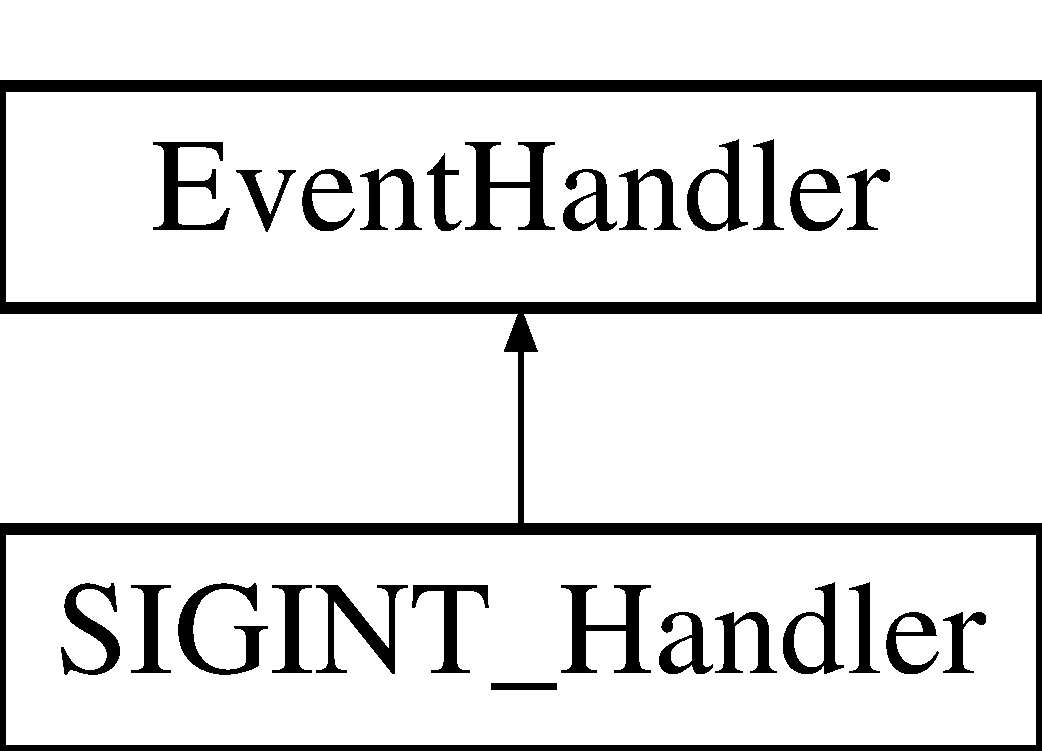
\includegraphics[height=2.000000cm]{classEventHandler}
\end{center}
\end{figure}
\subsection*{Public Member Functions}
\begin{DoxyCompactItemize}
\item 
\hypertarget{classEventHandler_a264a530841176ce475d7638dc78f1f2f}{virtual int {\bfseries handle\-Signal} (int signum)=0}\label{classEventHandler_a264a530841176ce475d7638dc78f1f2f}

\end{DoxyCompactItemize}


The documentation for this class was generated from the following file\-:\begin{DoxyCompactItemize}
\item 
Event\-Handler.\-h\end{DoxyCompactItemize}

\hypertarget{classLoggero}{\section{Loggero Class Reference}
\label{classLoggero}\index{Loggero@{Loggero}}
}
\subsection*{Public Member Functions}
\begin{DoxyCompactItemize}
\item 
int \hyperlink{classLoggero_af560ec1e9fc12d441d9539f1e939bf43}{log} (int type, string message)
\end{DoxyCompactItemize}
\subsection*{Static Public Member Functions}
\begin{DoxyCompactItemize}
\item 
static \hyperlink{classLoggero}{Loggero} $\ast$ \hyperlink{classLoggero_a0d827dcfffe0c6765f7ca9da856c3f06}{get\-Instnce} ()
\end{DoxyCompactItemize}


\subsection{Member Function Documentation}
\hypertarget{classLoggero_a0d827dcfffe0c6765f7ca9da856c3f06}{\index{Loggero@{Loggero}!get\-Instnce@{get\-Instnce}}
\index{get\-Instnce@{get\-Instnce}!Loggero@{Loggero}}
\subsubsection[{get\-Instnce}]{\setlength{\rightskip}{0pt plus 5cm}{\bf Loggero} $\ast$ Loggero\-::get\-Instnce (
\begin{DoxyParamCaption}
{}
\end{DoxyParamCaption}
)\hspace{0.3cm}{\ttfamily [static]}}}\label{classLoggero_a0d827dcfffe0c6765f7ca9da856c3f06}
\begin{DoxyReturn}{Returns}
the instance of the singleton \hyperlink{classLoggero}{Loggero} 
\end{DoxyReturn}
\hypertarget{classLoggero_af560ec1e9fc12d441d9539f1e939bf43}{\index{Loggero@{Loggero}!log@{log}}
\index{log@{log}!Loggero@{Loggero}}
\subsubsection[{log}]{\setlength{\rightskip}{0pt plus 5cm}int Loggero\-::log (
\begin{DoxyParamCaption}
\item[{int}]{type, }
\item[{string}]{message}
\end{DoxyParamCaption}
)}}\label{classLoggero_af560ec1e9fc12d441d9539f1e939bf43}

\begin{DoxyParams}{Parameters}
{\em type} & of log. See \hyperlink{classConstants}{Constants} \\
\hline
{\em message} & the message to log \\
\hline
\end{DoxyParams}
\begin{DoxyReturn}{Returns}
1 in error, 0 in success 
\end{DoxyReturn}


The documentation for this class was generated from the following files\-:\begin{DoxyCompactItemize}
\item 
Loggero.\-h\item 
Loggero.\-cpp\end{DoxyCompactItemize}

\hypertarget{classMessage}{\section{Message Class Reference}
\label{classMessage}\index{Message@{Message}}
}
\subsection*{Public Member Functions}
\begin{DoxyCompactItemize}
\item 
\hyperlink{classMessage_a3d631e5f5506a662dbff5f8a4469b279}{Message} (\hyperlink{classUser}{User} $\ast$emisor, \hyperlink{classUser}{User} $\ast$receptor, string body)
\item 
\hyperlink{classMessage_a763bb4ea8a99e1630a6e73653b7ace0a}{Message} (Json\-::\-Value)
\item 
const string \& \hyperlink{classMessage_a1de1dc1dd23372bc59d35eb65122e990}{get\-Body} () const 
\item 
string \hyperlink{classMessage_af85a5ded7c2ecbb967233d8d8ab12a64}{get\-Datetime} () const 
\item 
\hyperlink{classUser}{User} $\ast$ \hyperlink{classMessage_a6ef2c26162ee365b1ea7cc409bd3309c}{get\-Emisor} ()
\item 
\hyperlink{classUser}{User} $\ast$ \hyperlink{classMessage_a09b657e492505dead601b2fb2b46603c}{get\-Receptor} ()
\item 
void \hyperlink{classMessage_a3b5192fefe4e3aecef9490c3453e320e}{set\-Receptor} (\hyperlink{classUser}{User} $\ast$u)
\item 
Value \hyperlink{classMessage_a3239717cb012db702953305a548ad39b}{to\-Json\-Value} ()
\item 
string \hyperlink{classMessage_afdf05aa8cf0c9fad537c281960215c13}{to\-Json\-String} ()
\item 
string \hyperlink{classMessage_aaaaaa629aa85124152901e258ceedd69}{get\-Id} ()
\item 
void \hyperlink{classMessage_a657cdc286b04496c023998937de8c893}{set\-Id} (string id)
\end{DoxyCompactItemize}


\subsection{Constructor \& Destructor Documentation}
\hypertarget{classMessage_a3d631e5f5506a662dbff5f8a4469b279}{\index{Message@{Message}!Message@{Message}}
\index{Message@{Message}!Message@{Message}}
\subsubsection[{Message}]{\setlength{\rightskip}{0pt plus 5cm}Message\-::\-Message (
\begin{DoxyParamCaption}
\item[{{\bf User} $\ast$}]{emisor, }
\item[{{\bf User} $\ast$}]{receptor, }
\item[{string}]{body}
\end{DoxyParamCaption}
)}}\label{classMessage_a3d631e5f5506a662dbff5f8a4469b279}

\begin{DoxyParams}{Parameters}
{\em emisor} & a pointer to the user that sends the message \\
\hline
{\em receptor} & a pointer to the user that receives the message \\
\hline
{\em body} & string. \\
\hline
\end{DoxyParams}
\hypertarget{classMessage_a763bb4ea8a99e1630a6e73653b7ace0a}{\index{Message@{Message}!Message@{Message}}
\index{Message@{Message}!Message@{Message}}
\subsubsection[{Message}]{\setlength{\rightskip}{0pt plus 5cm}Message\-::\-Message (
\begin{DoxyParamCaption}
\item[{Json\-::\-Value}]{value}
\end{DoxyParamCaption}
)}}\label{classMessage_a763bb4ea8a99e1630a6e73653b7ace0a}

\begin{DoxyParams}{Parameters}
{\em value} & a Json\-::\-Value that represents the message \\
\hline
\end{DoxyParams}


\subsection{Member Function Documentation}
\hypertarget{classMessage_a1de1dc1dd23372bc59d35eb65122e990}{\index{Message@{Message}!get\-Body@{get\-Body}}
\index{get\-Body@{get\-Body}!Message@{Message}}
\subsubsection[{get\-Body}]{\setlength{\rightskip}{0pt plus 5cm}const string \& Message\-::get\-Body (
\begin{DoxyParamCaption}
{}
\end{DoxyParamCaption}
) const}}\label{classMessage_a1de1dc1dd23372bc59d35eb65122e990}
\begin{DoxyReturn}{Returns}
the body of the message as string 
\end{DoxyReturn}
\hypertarget{classMessage_af85a5ded7c2ecbb967233d8d8ab12a64}{\index{Message@{Message}!get\-Datetime@{get\-Datetime}}
\index{get\-Datetime@{get\-Datetime}!Message@{Message}}
\subsubsection[{get\-Datetime}]{\setlength{\rightskip}{0pt plus 5cm}string Message\-::get\-Datetime (
\begin{DoxyParamCaption}
{}
\end{DoxyParamCaption}
) const}}\label{classMessage_af85a5ded7c2ecbb967233d8d8ab12a64}
\begin{DoxyReturn}{Returns}
the datetime of the message as string 
\end{DoxyReturn}
\hypertarget{classMessage_a6ef2c26162ee365b1ea7cc409bd3309c}{\index{Message@{Message}!get\-Emisor@{get\-Emisor}}
\index{get\-Emisor@{get\-Emisor}!Message@{Message}}
\subsubsection[{get\-Emisor}]{\setlength{\rightskip}{0pt plus 5cm}{\bf User} $\ast$ Message\-::get\-Emisor (
\begin{DoxyParamCaption}
{}
\end{DoxyParamCaption}
)}}\label{classMessage_a6ef2c26162ee365b1ea7cc409bd3309c}
\begin{DoxyReturn}{Returns}
a pointer to the user that sends the message 
\end{DoxyReturn}
\hypertarget{classMessage_aaaaaa629aa85124152901e258ceedd69}{\index{Message@{Message}!get\-Id@{get\-Id}}
\index{get\-Id@{get\-Id}!Message@{Message}}
\subsubsection[{get\-Id}]{\setlength{\rightskip}{0pt plus 5cm}string Message\-::get\-Id (
\begin{DoxyParamCaption}
{}
\end{DoxyParamCaption}
)}}\label{classMessage_aaaaaa629aa85124152901e258ceedd69}
\begin{DoxyReturn}{Returns}
a string that is the id of the message 
\end{DoxyReturn}
\hypertarget{classMessage_a09b657e492505dead601b2fb2b46603c}{\index{Message@{Message}!get\-Receptor@{get\-Receptor}}
\index{get\-Receptor@{get\-Receptor}!Message@{Message}}
\subsubsection[{get\-Receptor}]{\setlength{\rightskip}{0pt plus 5cm}{\bf User} $\ast$ Message\-::get\-Receptor (
\begin{DoxyParamCaption}
{}
\end{DoxyParamCaption}
)}}\label{classMessage_a09b657e492505dead601b2fb2b46603c}
\begin{DoxyReturn}{Returns}
a pointer to the user that receives the message 
\end{DoxyReturn}
\hypertarget{classMessage_a657cdc286b04496c023998937de8c893}{\index{Message@{Message}!set\-Id@{set\-Id}}
\index{set\-Id@{set\-Id}!Message@{Message}}
\subsubsection[{set\-Id}]{\setlength{\rightskip}{0pt plus 5cm}void Message\-::set\-Id (
\begin{DoxyParamCaption}
\item[{string}]{id}
\end{DoxyParamCaption}
)}}\label{classMessage_a657cdc286b04496c023998937de8c893}

\begin{DoxyParams}{Parameters}
{\em id} & a string that is the id of the message \\
\hline
\end{DoxyParams}
\hypertarget{classMessage_a3b5192fefe4e3aecef9490c3453e320e}{\index{Message@{Message}!set\-Receptor@{set\-Receptor}}
\index{set\-Receptor@{set\-Receptor}!Message@{Message}}
\subsubsection[{set\-Receptor}]{\setlength{\rightskip}{0pt plus 5cm}void Message\-::set\-Receptor (
\begin{DoxyParamCaption}
\item[{{\bf User} $\ast$}]{u}
\end{DoxyParamCaption}
)}}\label{classMessage_a3b5192fefe4e3aecef9490c3453e320e}

\begin{DoxyParams}{Parameters}
{\em u} & a pointer to the user that receives the message \\
\hline
\end{DoxyParams}
\hypertarget{classMessage_afdf05aa8cf0c9fad537c281960215c13}{\index{Message@{Message}!to\-Json\-String@{to\-Json\-String}}
\index{to\-Json\-String@{to\-Json\-String}!Message@{Message}}
\subsubsection[{to\-Json\-String}]{\setlength{\rightskip}{0pt plus 5cm}string Message\-::to\-Json\-String (
\begin{DoxyParamCaption}
{}
\end{DoxyParamCaption}
)}}\label{classMessage_afdf05aa8cf0c9fad537c281960215c13}
\begin{DoxyReturn}{Returns}
a json string of the message 
\end{DoxyReturn}
\hypertarget{classMessage_a3239717cb012db702953305a548ad39b}{\index{Message@{Message}!to\-Json\-Value@{to\-Json\-Value}}
\index{to\-Json\-Value@{to\-Json\-Value}!Message@{Message}}
\subsubsection[{to\-Json\-Value}]{\setlength{\rightskip}{0pt plus 5cm}Value Message\-::to\-Json\-Value (
\begin{DoxyParamCaption}
{}
\end{DoxyParamCaption}
)}}\label{classMessage_a3239717cb012db702953305a548ad39b}
\begin{DoxyReturn}{Returns}
a Json\-::\-Value of the message 
\end{DoxyReturn}


The documentation for this class was generated from the following files\-:\begin{DoxyCompactItemize}
\item 
Message.\-h\item 
Message.\-cpp\end{DoxyCompactItemize}

\hypertarget{classMessageFactory}{\section{Message\-Factory Class Reference}
\label{classMessageFactory}\index{Message\-Factory@{Message\-Factory}}
}
\subsection*{Static Public Member Functions}
\begin{DoxyCompactItemize}
\item 
static \hyperlink{classMessage}{Message} $\ast$ \hyperlink{classMessageFactory_a4e26f5e4948862fcef2501a00634861b}{create\-Message} (Json\-::\-Value value)
\end{DoxyCompactItemize}


\subsection{Member Function Documentation}
\hypertarget{classMessageFactory_a4e26f5e4948862fcef2501a00634861b}{\index{Message\-Factory@{Message\-Factory}!create\-Message@{create\-Message}}
\index{create\-Message@{create\-Message}!MessageFactory@{Message\-Factory}}
\subsubsection[{create\-Message}]{\setlength{\rightskip}{0pt plus 5cm}{\bf Message} $\ast$ Message\-Factory\-::create\-Message (
\begin{DoxyParamCaption}
\item[{Json\-::\-Value}]{value}
\end{DoxyParamCaption}
)\hspace{0.3cm}{\ttfamily [static]}}}\label{classMessageFactory_a4e26f5e4948862fcef2501a00634861b}

\begin{DoxyParams}{Parameters}
{\em value} & a Json\-::\-Value that represents the message \\
\hline
\end{DoxyParams}
\begin{DoxyReturn}{Returns}
a pointer to the message 
\end{DoxyReturn}


The documentation for this class was generated from the following files\-:\begin{DoxyCompactItemize}
\item 
Message\-Factory.\-h\item 
Message\-Factory.\-cpp\end{DoxyCompactItemize}

\hypertarget{classProceso}{\section{Proceso Class Reference}
\label{classProceso}\index{Proceso@{Proceso}}
}
Inheritance diagram for Proceso\-:\begin{figure}[H]
\begin{center}
\leavevmode
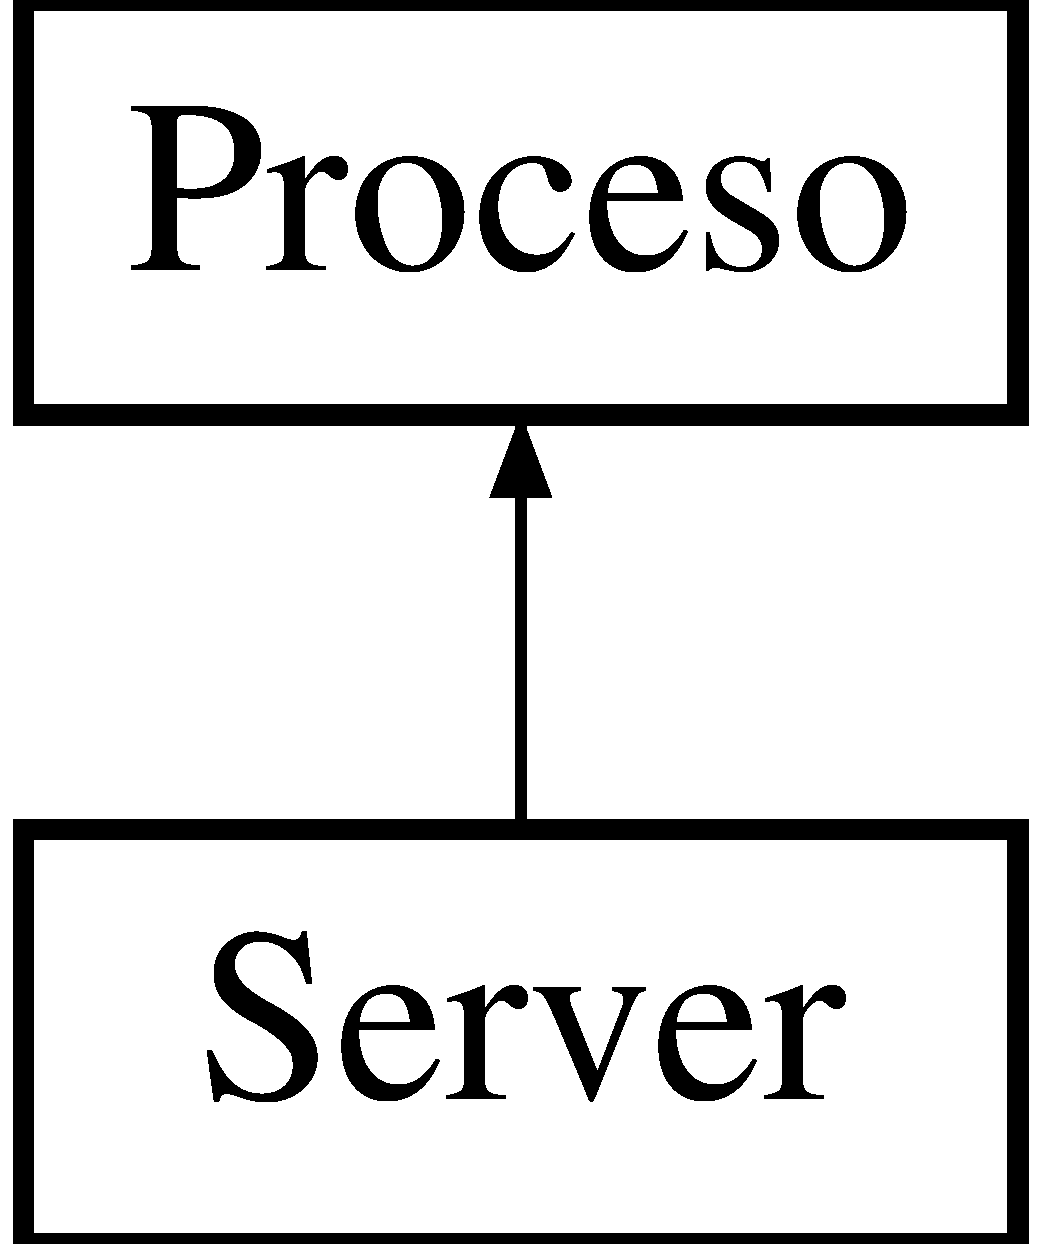
\includegraphics[height=2.000000cm]{classProceso}
\end{center}
\end{figure}
\subsection*{Public Attributes}
\begin{DoxyCompactItemize}
\item 
\hypertarget{classProceso_affb17981ef18a4892dd81eac428ab4a9}{\hyperlink{classSIGINT__Handler}{S\-I\-G\-I\-N\-T\-\_\-\-Handler} {\bfseries sigint\-\_\-handler}}\label{classProceso_affb17981ef18a4892dd81eac428ab4a9}

\end{DoxyCompactItemize}


The documentation for this class was generated from the following files\-:\begin{DoxyCompactItemize}
\item 
Proceso.\-h\item 
Proceso.\-cpp\end{DoxyCompactItemize}

\hypertarget{classServer}{\section{Server Class Reference}
\label{classServer}\index{Server@{Server}}
}
Inheritance diagram for Server\-:\begin{figure}[H]
\begin{center}
\leavevmode
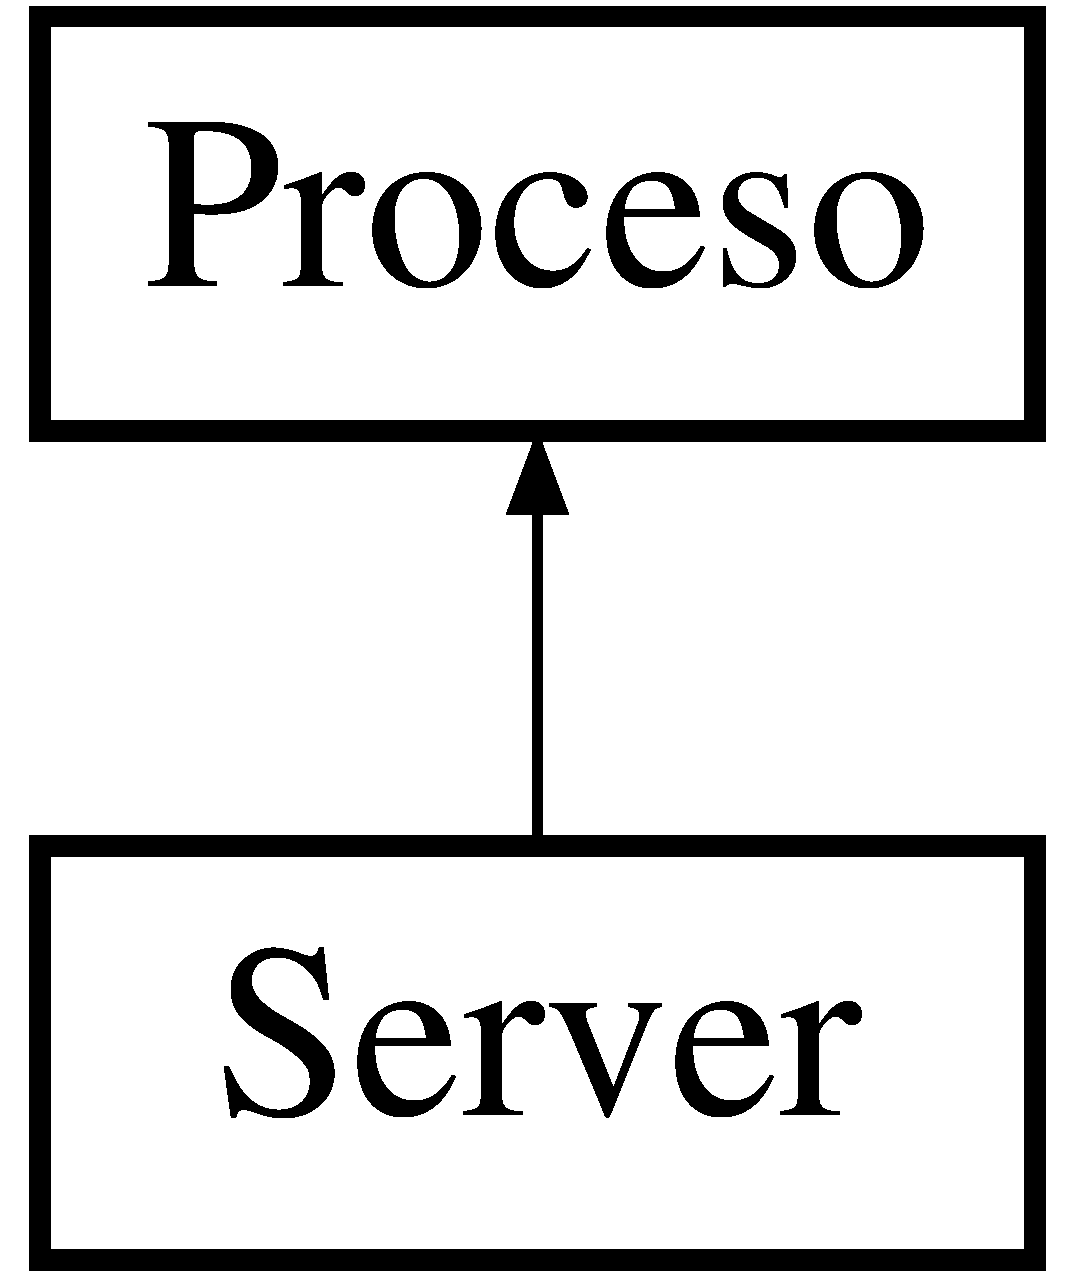
\includegraphics[height=2.000000cm]{classServer}
\end{center}
\end{figure}
\subsection*{Public Member Functions}
\begin{DoxyCompactItemize}
\item 
\hypertarget{classServer_abb27d30b40a94326e3fd629d3b30b7d5}{void {\bfseries run} ()}\label{classServer_abb27d30b40a94326e3fd629d3b30b7d5}

\item 
int \hyperlink{classServer_a35ee7138b8d6f2aea6ecaf63dc874441}{ev\-\_\-handler} (mg\-\_\-connection $\ast$conn, enum mg\-\_\-event ev)
\end{DoxyCompactItemize}
\subsection*{Additional Inherited Members}


\subsection{Member Function Documentation}
\hypertarget{classServer_a35ee7138b8d6f2aea6ecaf63dc874441}{\index{Server@{Server}!ev\-\_\-handler@{ev\-\_\-handler}}
\index{ev\-\_\-handler@{ev\-\_\-handler}!Server@{Server}}
\subsubsection[{ev\-\_\-handler}]{\setlength{\rightskip}{0pt plus 5cm}int Server\-::ev\-\_\-handler (
\begin{DoxyParamCaption}
\item[{mg\-\_\-connection $\ast$}]{conn, }
\item[{enum mg\-\_\-event}]{ev}
\end{DoxyParamCaption}
)}}\label{classServer_a35ee7138b8d6f2aea6ecaf63dc874441}

\begin{DoxyParams}{Parameters}
{\em conn} & \\
\hline
{\em ev} & \\
\hline
\end{DoxyParams}
\begin{DoxyReturn}{Returns}

\end{DoxyReturn}


The documentation for this class was generated from the following files\-:\begin{DoxyCompactItemize}
\item 
Server.\-h\item 
Server.\-cpp\end{DoxyCompactItemize}

\hypertarget{classServiceLayer}{\section{Service\-Layer Class Reference}
\label{classServiceLayer}\index{Service\-Layer@{Service\-Layer}}
}
\subsection*{Public Member Functions}
\begin{DoxyCompactItemize}
\item 
\hypertarget{classServiceLayer_a5c564934fe9abbc2d0106f84641d1636}{\hyperlink{classDatabase}{Database} $\ast$ {\bfseries get\-Database} ()}\label{classServiceLayer_a5c564934fe9abbc2d0106f84641d1636}

\item 
string \hyperlink{classServiceLayer_a156db9a26ee9c18b5dc004a53e6db135}{login} (string username, string password)
\item 
string \hyperlink{classServiceLayer_aa58f32a68f65731f5bff417a6d8587cd}{logout} (string username, string token)
\item 
string \hyperlink{classServiceLayer_a3158abab790bb26288e3d42529044c47}{validate\-Token} (string username, string token)
\item 
string \hyperlink{classServiceLayer_ae7b18cf7b281a5e97fe291202865bf24}{create\-User} (string json)
\item 
string \hyperlink{classServiceLayer_a8b160670006abd96a72634c021ff171f}{send\-Message} (string username, string token, string json)
\item 
string \hyperlink{classServiceLayer_a7b502342d937cb644ad8fa077cf4c563}{get\-Conversations} (string username, string token)
\item 
string \hyperlink{classServiceLayer_a3d5142f67a7d93a9b190c742772033d1}{get\-Messages} (string username, string token, string user2)
\item 
string \hyperlink{classServiceLayer_afe132fdef6f03f5f62caa525e4327100}{get\-User\-Profile} (string username, string token, string user\-To\-Visit)
\item 
string \hyperlink{classServiceLayer_aa734255db70314f738b097b6c048c994}{get\-Users\-Profile} (string username, string token)
\item 
string \hyperlink{classServiceLayer_a927f11b4f38d260b83b3c4de67801d81}{update\-Profile} (string username, string token, string data)
\end{DoxyCompactItemize}
\subsection*{Static Public Attributes}
\begin{DoxyCompactItemize}
\item 
\hypertarget{classServiceLayer_a958d3259dc9d8b7db628f671ac2b8c64}{static string {\bfseries E\-R\-R\-O\-R\-\_\-\-S\-T\-R\-I\-N\-G} = \char`\"{}E\-R\-R\-O\-R\char`\"{}}\label{classServiceLayer_a958d3259dc9d8b7db628f671ac2b8c64}

\item 
\hypertarget{classServiceLayer_a5109f9280872623944c8529af6992810}{static string {\bfseries O\-K\-\_\-\-S\-T\-R\-I\-N\-G} = \char`\"{}O\-K\char`\"{}}\label{classServiceLayer_a5109f9280872623944c8529af6992810}

\item 
\hypertarget{classServiceLayer_aeef05f74f4820e27835bbd7b5bba38f1}{static int {\bfseries I\-N\-V\-A\-L\-I\-D\-\_\-\-U\-S\-E\-R\-N\-A\-M\-E} = 1}\label{classServiceLayer_aeef05f74f4820e27835bbd7b5bba38f1}

\item 
\hypertarget{classServiceLayer_af48302af91d1b5f9198cc4b39ca747b2}{static int {\bfseries I\-N\-V\-A\-L\-I\-D\-\_\-\-P\-A\-S\-S\-W\-O\-R\-D} = 2}\label{classServiceLayer_af48302af91d1b5f9198cc4b39ca747b2}

\item 
\hypertarget{classServiceLayer_a2b7a685fc838d437c6da8e09bfbd3093}{static int {\bfseries I\-N\-V\-A\-L\-I\-D\-\_\-\-T\-O\-K\-E\-N} = 3}\label{classServiceLayer_a2b7a685fc838d437c6da8e09bfbd3093}

\item 
\hypertarget{classServiceLayer_a1165582032762224096a72ce3b9a026d}{static int {\bfseries E\-R\-R\-O\-R\-\_\-\-S\-E\-N\-D\-\_\-\-M\-E\-S\-S\-A\-G\-E} = 4}\label{classServiceLayer_a1165582032762224096a72ce3b9a026d}

\item 
\hypertarget{classServiceLayer_a158c78456324a5914d012a90506e2d98}{static int {\bfseries E\-R\-R\-O\-R\-\_\-\-U\-S\-E\-R\-\_\-\-P\-R\-O\-F\-I\-L\-E\-\_\-\-D\-O\-E\-S\-N\-T\-\_\-\-E\-X\-I\-S\-T\-S} = 5}\label{classServiceLayer_a158c78456324a5914d012a90506e2d98}

\item 
\hypertarget{classServiceLayer_ad6f2c41aad09560a4fe86777ffa75289}{static int {\bfseries N\-O\-\_\-\-U\-S\-E\-R\-N\-A\-M\-E} = 8}\label{classServiceLayer_ad6f2c41aad09560a4fe86777ffa75289}

\item 
\hypertarget{classServiceLayer_ab4e8306edb3904639e9884ff1d48578c}{static int {\bfseries N\-O\-\_\-\-P\-A\-S\-S\-W\-O\-R\-D} = 7}\label{classServiceLayer_ab4e8306edb3904639e9884ff1d48578c}

\item 
\hypertarget{classServiceLayer_adb5e8613d24bf9634b568f2958fbcb96}{static int {\bfseries U\-S\-E\-R\-N\-A\-M\-E\-\_\-\-A\-L\-R\-E\-A\-D\-Y\-\_\-\-E\-X\-I\-S\-T\-S} = 6}\label{classServiceLayer_adb5e8613d24bf9634b568f2958fbcb96}

\item 
\hypertarget{classServiceLayer_a3b13f26199c41e3fc09ecc6c9d44b604}{static int {\bfseries I\-N\-V\-A\-L\-I\-D\-\_\-\-J\-S\-O\-N} = 9}\label{classServiceLayer_a3b13f26199c41e3fc09ecc6c9d44b604}

\item 
\hypertarget{classServiceLayer_a2138d03937561da9c364c93bef98879b}{static int {\bfseries E\-R\-R\-O\-R\-\_\-\-O\-N\-\_\-\-S\-A\-V\-E} = 10}\label{classServiceLayer_a2138d03937561da9c364c93bef98879b}

\end{DoxyCompactItemize}


\subsection{Member Function Documentation}
\hypertarget{classServiceLayer_ae7b18cf7b281a5e97fe291202865bf24}{\index{Service\-Layer@{Service\-Layer}!create\-User@{create\-User}}
\index{create\-User@{create\-User}!ServiceLayer@{Service\-Layer}}
\subsubsection[{create\-User}]{\setlength{\rightskip}{0pt plus 5cm}string Service\-Layer\-::create\-User (
\begin{DoxyParamCaption}
\item[{string}]{json}
\end{DoxyParamCaption}
)}}\label{classServiceLayer_ae7b18cf7b281a5e97fe291202865bf24}

\begin{DoxyParams}{Parameters}
{\em json} & \\
\hline
\end{DoxyParams}
\begin{DoxyReturn}{Returns}

\end{DoxyReturn}
\hypertarget{classServiceLayer_a7b502342d937cb644ad8fa077cf4c563}{\index{Service\-Layer@{Service\-Layer}!get\-Conversations@{get\-Conversations}}
\index{get\-Conversations@{get\-Conversations}!ServiceLayer@{Service\-Layer}}
\subsubsection[{get\-Conversations}]{\setlength{\rightskip}{0pt plus 5cm}string Service\-Layer\-::get\-Conversations (
\begin{DoxyParamCaption}
\item[{string}]{username, }
\item[{string}]{token}
\end{DoxyParamCaption}
)}}\label{classServiceLayer_a7b502342d937cb644ad8fa077cf4c563}

\begin{DoxyParams}{Parameters}
{\em username} & \\
\hline
{\em token} & \\
\hline
\end{DoxyParams}
\begin{DoxyReturn}{Returns}

\end{DoxyReturn}
\hypertarget{classServiceLayer_a3d5142f67a7d93a9b190c742772033d1}{\index{Service\-Layer@{Service\-Layer}!get\-Messages@{get\-Messages}}
\index{get\-Messages@{get\-Messages}!ServiceLayer@{Service\-Layer}}
\subsubsection[{get\-Messages}]{\setlength{\rightskip}{0pt plus 5cm}string Service\-Layer\-::get\-Messages (
\begin{DoxyParamCaption}
\item[{string}]{username, }
\item[{string}]{token, }
\item[{string}]{user2}
\end{DoxyParamCaption}
)}}\label{classServiceLayer_a3d5142f67a7d93a9b190c742772033d1}

\begin{DoxyParams}{Parameters}
{\em username} & \\
\hline
{\em token} & \\
\hline
{\em user2} & \\
\hline
\end{DoxyParams}
\begin{DoxyReturn}{Returns}

\end{DoxyReturn}
\hypertarget{classServiceLayer_afe132fdef6f03f5f62caa525e4327100}{\index{Service\-Layer@{Service\-Layer}!get\-User\-Profile@{get\-User\-Profile}}
\index{get\-User\-Profile@{get\-User\-Profile}!ServiceLayer@{Service\-Layer}}
\subsubsection[{get\-User\-Profile}]{\setlength{\rightskip}{0pt plus 5cm}string Service\-Layer\-::get\-User\-Profile (
\begin{DoxyParamCaption}
\item[{string}]{username, }
\item[{string}]{token, }
\item[{string}]{user\-To\-Visit}
\end{DoxyParamCaption}
)}}\label{classServiceLayer_afe132fdef6f03f5f62caa525e4327100}

\begin{DoxyParams}{Parameters}
{\em username} & \\
\hline
{\em token} & \\
\hline
{\em user\-To\-Visit} & \\
\hline
\end{DoxyParams}
\begin{DoxyReturn}{Returns}

\end{DoxyReturn}
\hypertarget{classServiceLayer_aa734255db70314f738b097b6c048c994}{\index{Service\-Layer@{Service\-Layer}!get\-Users\-Profile@{get\-Users\-Profile}}
\index{get\-Users\-Profile@{get\-Users\-Profile}!ServiceLayer@{Service\-Layer}}
\subsubsection[{get\-Users\-Profile}]{\setlength{\rightskip}{0pt plus 5cm}string Service\-Layer\-::get\-Users\-Profile (
\begin{DoxyParamCaption}
\item[{string}]{username, }
\item[{string}]{token}
\end{DoxyParamCaption}
)}}\label{classServiceLayer_aa734255db70314f738b097b6c048c994}

\begin{DoxyParams}{Parameters}
{\em username} & \\
\hline
{\em token} & \\
\hline
\end{DoxyParams}
\begin{DoxyReturn}{Returns}

\end{DoxyReturn}
\hypertarget{classServiceLayer_a156db9a26ee9c18b5dc004a53e6db135}{\index{Service\-Layer@{Service\-Layer}!login@{login}}
\index{login@{login}!ServiceLayer@{Service\-Layer}}
\subsubsection[{login}]{\setlength{\rightskip}{0pt plus 5cm}string Service\-Layer\-::login (
\begin{DoxyParamCaption}
\item[{string}]{username, }
\item[{string}]{password}
\end{DoxyParamCaption}
)}}\label{classServiceLayer_a156db9a26ee9c18b5dc004a53e6db135}

\begin{DoxyParams}{Parameters}
{\em username} & \\
\hline
{\em password} & \\
\hline
\end{DoxyParams}
\begin{DoxyReturn}{Returns}

\end{DoxyReturn}
\hypertarget{classServiceLayer_aa58f32a68f65731f5bff417a6d8587cd}{\index{Service\-Layer@{Service\-Layer}!logout@{logout}}
\index{logout@{logout}!ServiceLayer@{Service\-Layer}}
\subsubsection[{logout}]{\setlength{\rightskip}{0pt plus 5cm}string Service\-Layer\-::logout (
\begin{DoxyParamCaption}
\item[{string}]{username, }
\item[{string}]{token}
\end{DoxyParamCaption}
)}}\label{classServiceLayer_aa58f32a68f65731f5bff417a6d8587cd}

\begin{DoxyParams}{Parameters}
{\em username} & \\
\hline
{\em token} & \\
\hline
\end{DoxyParams}
\begin{DoxyReturn}{Returns}

\end{DoxyReturn}
\hypertarget{classServiceLayer_a8b160670006abd96a72634c021ff171f}{\index{Service\-Layer@{Service\-Layer}!send\-Message@{send\-Message}}
\index{send\-Message@{send\-Message}!ServiceLayer@{Service\-Layer}}
\subsubsection[{send\-Message}]{\setlength{\rightskip}{0pt plus 5cm}string Service\-Layer\-::send\-Message (
\begin{DoxyParamCaption}
\item[{string}]{username, }
\item[{string}]{token, }
\item[{string}]{json\-Message}
\end{DoxyParamCaption}
)}}\label{classServiceLayer_a8b160670006abd96a72634c021ff171f}

\begin{DoxyParams}{Parameters}
{\em username} & \\
\hline
{\em token} & \\
\hline
{\em json\-Message} & \\
\hline
\end{DoxyParams}
\begin{DoxyReturn}{Returns}

\end{DoxyReturn}
\hypertarget{classServiceLayer_a927f11b4f38d260b83b3c4de67801d81}{\index{Service\-Layer@{Service\-Layer}!update\-Profile@{update\-Profile}}
\index{update\-Profile@{update\-Profile}!ServiceLayer@{Service\-Layer}}
\subsubsection[{update\-Profile}]{\setlength{\rightskip}{0pt plus 5cm}string Service\-Layer\-::update\-Profile (
\begin{DoxyParamCaption}
\item[{string}]{username, }
\item[{string}]{token, }
\item[{string}]{data}
\end{DoxyParamCaption}
)}}\label{classServiceLayer_a927f11b4f38d260b83b3c4de67801d81}

\begin{DoxyParams}{Parameters}
{\em username} & \\
\hline
{\em token} & \\
\hline
{\em data} & \\
\hline
\end{DoxyParams}
\begin{DoxyReturn}{Returns}

\end{DoxyReturn}
\hypertarget{classServiceLayer_a3158abab790bb26288e3d42529044c47}{\index{Service\-Layer@{Service\-Layer}!validate\-Token@{validate\-Token}}
\index{validate\-Token@{validate\-Token}!ServiceLayer@{Service\-Layer}}
\subsubsection[{validate\-Token}]{\setlength{\rightskip}{0pt plus 5cm}string Service\-Layer\-::validate\-Token (
\begin{DoxyParamCaption}
\item[{string}]{username, }
\item[{string}]{token}
\end{DoxyParamCaption}
)}}\label{classServiceLayer_a3158abab790bb26288e3d42529044c47}

\begin{DoxyParams}{Parameters}
{\em username} & \\
\hline
{\em token} & \\
\hline
\end{DoxyParams}
\begin{DoxyReturn}{Returns}

\end{DoxyReturn}


The documentation for this class was generated from the following files\-:\begin{DoxyCompactItemize}
\item 
Service\-Layer.\-h\item 
Service\-Layer.\-cpp\end{DoxyCompactItemize}

\hypertarget{classSIGINT__Handler}{\section{S\-I\-G\-I\-N\-T\-\_\-\-Handler Class Reference}
\label{classSIGINT__Handler}\index{S\-I\-G\-I\-N\-T\-\_\-\-Handler@{S\-I\-G\-I\-N\-T\-\_\-\-Handler}}
}
Inheritance diagram for S\-I\-G\-I\-N\-T\-\_\-\-Handler\-:\begin{figure}[H]
\begin{center}
\leavevmode
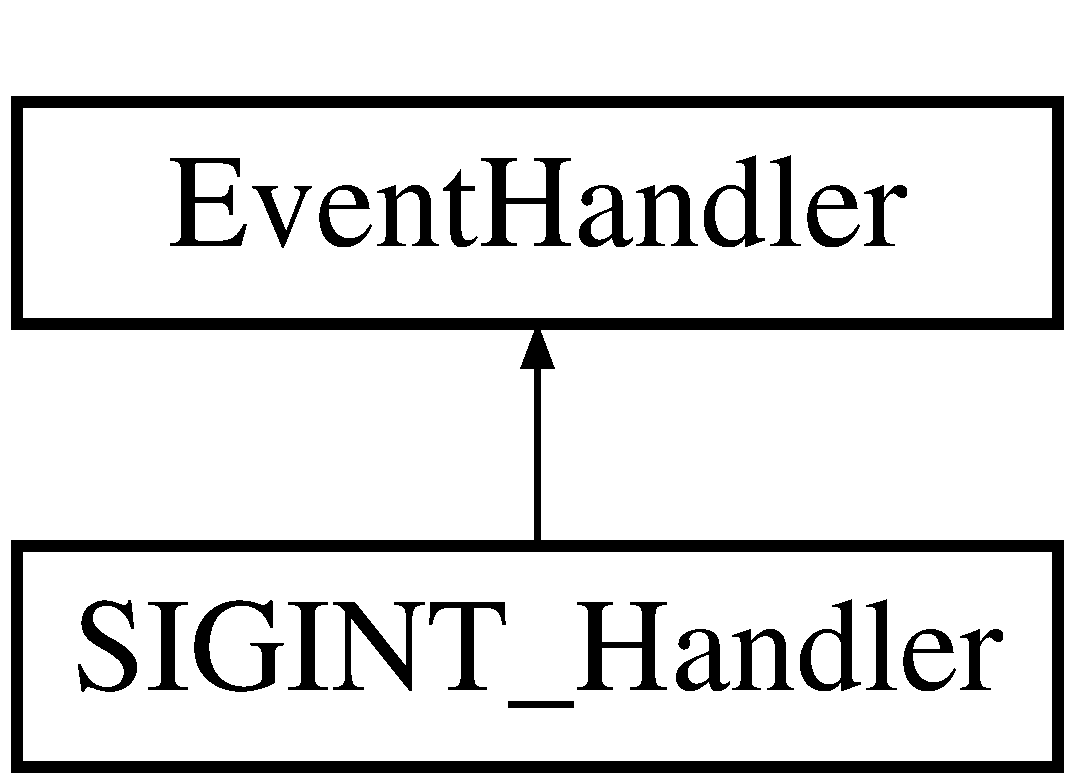
\includegraphics[height=2.000000cm]{classSIGINT__Handler}
\end{center}
\end{figure}
\subsection*{Public Member Functions}
\begin{DoxyCompactItemize}
\item 
\hypertarget{classSIGINT__Handler_a0bac7e6d02c1fb09c9795c5282b1c98a}{virtual int {\bfseries handle\-Signal} (int signum)}\label{classSIGINT__Handler_a0bac7e6d02c1fb09c9795c5282b1c98a}

\item 
\hypertarget{classSIGINT__Handler_a0e63db035673b15d289c45076f54f682}{sig\-\_\-atomic\-\_\-t {\bfseries get\-Graceful\-Quit} () const }\label{classSIGINT__Handler_a0e63db035673b15d289c45076f54f682}

\end{DoxyCompactItemize}


The documentation for this class was generated from the following file\-:\begin{DoxyCompactItemize}
\item 
S\-I\-G\-I\-N\-T\-\_\-\-Handler.\-h\end{DoxyCompactItemize}

\hypertarget{classSignalHandler}{\section{Signal\-Handler Class Reference}
\label{classSignalHandler}\index{Signal\-Handler@{Signal\-Handler}}
}
\subsection*{Public Member Functions}
\begin{DoxyCompactItemize}
\item 
\hypertarget{classSignalHandler_a41a15d866eed0c4df9ef8f685ce4d6a7}{\hyperlink{classEventHandler}{Event\-Handler} $\ast$ {\bfseries registrar\-Handler} (int signum, \hyperlink{classEventHandler}{Event\-Handler} $\ast$eh)}\label{classSignalHandler_a41a15d866eed0c4df9ef8f685ce4d6a7}

\end{DoxyCompactItemize}
\subsection*{Static Public Member Functions}
\begin{DoxyCompactItemize}
\item 
\hypertarget{classSignalHandler_a753799244d13e9c998e8b6c7696f4b91}{static \hyperlink{classSignalHandler}{Signal\-Handler} $\ast$ {\bfseries get\-Instance} ()}\label{classSignalHandler_a753799244d13e9c998e8b6c7696f4b91}

\item 
\hypertarget{classSignalHandler_afae3c473d92a8a2c7bd29ee26078ee70}{static void {\bfseries destruir} ()}\label{classSignalHandler_afae3c473d92a8a2c7bd29ee26078ee70}

\end{DoxyCompactItemize}


The documentation for this class was generated from the following files\-:\begin{DoxyCompactItemize}
\item 
Signal\-Handler.\-h\item 
Signal\-Handler.\-cpp\end{DoxyCompactItemize}

\hypertarget{classUser}{\section{User Class Reference}
\label{classUser}\index{User@{User}}
}
\subsection*{Public Member Functions}
\begin{DoxyCompactItemize}
\item 
\hyperlink{classUser_a79cb2c4bc5ad9221a6e55b6a0981a27e}{User} (string username)
\item 
string \hyperlink{classUser_adb316ac38d5f62a967686e7b736a0469}{get\-Name} ()
\item 
void \hyperlink{classUser_ac44eb16e566dd060399e8f87ceec3fac}{set\-Name} (const string \&name)
\item 
bool \hyperlink{classUser_a73952dc0320736f3532e0037ae27cfef}{is\-Online} ()
\item 
void \hyperlink{classUser_a9cbe82e7191959323c3d380b6e78bf33}{set\-Online} (bool online)
\item 
string \hyperlink{classUser_a090eb9ee354cc25b2e8240b714b39d64}{get\-Password} ()
\item 
void \hyperlink{classUser_a00ba1579772decc59ab7f97bc262ce4a}{set\-Password} (const string \&password)
\item 
string \hyperlink{classUser_a5705c32c347050449ba6d72f32f18482}{get\-Username} ()
\item 
string \hyperlink{classUser_a700372bc6d19cbac725465de917b38a3}{get\-Token} ()
\item 
void \hyperlink{classUser_abc940c6478909bdf61acc5cfec24f189}{set\-Token} (string t)
\item 
string \hyperlink{classUser_abde67d56392ae39f8f9a47dae95f4220}{get\-Profile\-Image} ()
\item 
void \hyperlink{classUser_acc6da9f66ccdea972de126acadc3f69f}{set\-Profile\-Image} (string image)
\item 
double \hyperlink{classUser_a78ff4937b992a5a53c2fdc30be97507d}{get\-Latitud} ()
\item 
void \hyperlink{classUser_ad79d7b69bcf6e0b9070dcd539884d0f8}{set\-Latitud} (double latitud)
\item 
double \hyperlink{classUser_a811258c8bd9966d530297feb60619795}{get\-Longitud} ()
\item 
void \hyperlink{classUser_aafdb669757a37e09d56c412d69835144}{set\-Longitud} (double longitud)
\item 
string \hyperlink{classUser_a7d0456bd4a7f1a317e85fc3a58778541}{get\-Location} ()
\item 
void \hyperlink{classUser_aafccf6cd7fb08acde087389892d03f24}{set\-Location} (string location)
\item 
string \hyperlink{classUser_a70692f9ab9740a20d62f7086c4741e54}{get\-Checkin\-Datetime} ()
\item 
void \hyperlink{classUser_a3147b802b9e598b1d191b983115fefef}{set\-Checkin\-Datetime} (string datetime)
\item 
string \hyperlink{classUser_a92940ade2055d4582e847abb755eeef2}{get\-Last\-Activity\-Datetime} ()
\item 
void \hyperlink{classUser_a969006ba369cf770f0b23fb836033226}{set\-Last\-Activity\-Datetime} (string datetime)
\item 
void \hyperlink{classUser_a42fc61851c865d8e9e0a02dd6d794553}{login} ()
\item 
void \hyperlink{classUser_ade7eb5acf5097892168086ceed504ab3}{logout} ()
\item 
void \hyperlink{classUser_a416c9c7d90055844050106aa5b493471}{update\-User} (Json\-::\-Value val)
\item 
Json\-::\-Value \hyperlink{classUser_a130b4d4f3ba0a1641af4ad68f70e8711}{to\-Json\-Value} ()
\item 
string \hyperlink{classUser_aabc2c7838ee6a9950999112b45f657b7}{to\-Json\-String} ()
\item 
Json\-::\-Value \hyperlink{classUser_a7afe8d1e03e893b4da768773d4f444f8}{get\-User\-Profile\-Json\-Value} ()
\item 
Json\-::\-Value \hyperlink{classUser_a0bfa5d8db0a33ba1f8f69f617d697783}{get\-User\-Login\-Profile\-Json\-Value} ()
\end{DoxyCompactItemize}


\subsection{Constructor \& Destructor Documentation}
\hypertarget{classUser_a79cb2c4bc5ad9221a6e55b6a0981a27e}{\index{User@{User}!User@{User}}
\index{User@{User}!User@{User}}
\subsubsection[{User}]{\setlength{\rightskip}{0pt plus 5cm}User\-::\-User (
\begin{DoxyParamCaption}
\item[{string}]{username}
\end{DoxyParamCaption}
)}}\label{classUser_a79cb2c4bc5ad9221a6e55b6a0981a27e}

\begin{DoxyParams}{Parameters}
{\em username} & of the user as a string \\
\hline
\end{DoxyParams}


\subsection{Member Function Documentation}
\hypertarget{classUser_a70692f9ab9740a20d62f7086c4741e54}{\index{User@{User}!get\-Checkin\-Datetime@{get\-Checkin\-Datetime}}
\index{get\-Checkin\-Datetime@{get\-Checkin\-Datetime}!User@{User}}
\subsubsection[{get\-Checkin\-Datetime}]{\setlength{\rightskip}{0pt plus 5cm}string User\-::get\-Checkin\-Datetime (
\begin{DoxyParamCaption}
{}
\end{DoxyParamCaption}
)}}\label{classUser_a70692f9ab9740a20d62f7086c4741e54}
\begin{DoxyReturn}{Returns}
a string 
\end{DoxyReturn}
\hypertarget{classUser_a92940ade2055d4582e847abb755eeef2}{\index{User@{User}!get\-Last\-Activity\-Datetime@{get\-Last\-Activity\-Datetime}}
\index{get\-Last\-Activity\-Datetime@{get\-Last\-Activity\-Datetime}!User@{User}}
\subsubsection[{get\-Last\-Activity\-Datetime}]{\setlength{\rightskip}{0pt plus 5cm}string User\-::get\-Last\-Activity\-Datetime (
\begin{DoxyParamCaption}
{}
\end{DoxyParamCaption}
)}}\label{classUser_a92940ade2055d4582e847abb755eeef2}
\begin{DoxyReturn}{Returns}
a string 
\end{DoxyReturn}
\hypertarget{classUser_a78ff4937b992a5a53c2fdc30be97507d}{\index{User@{User}!get\-Latitud@{get\-Latitud}}
\index{get\-Latitud@{get\-Latitud}!User@{User}}
\subsubsection[{get\-Latitud}]{\setlength{\rightskip}{0pt plus 5cm}double User\-::get\-Latitud (
\begin{DoxyParamCaption}
{}
\end{DoxyParamCaption}
)}}\label{classUser_a78ff4937b992a5a53c2fdc30be97507d}
\begin{DoxyReturn}{Returns}
a double 
\end{DoxyReturn}
\hypertarget{classUser_a7d0456bd4a7f1a317e85fc3a58778541}{\index{User@{User}!get\-Location@{get\-Location}}
\index{get\-Location@{get\-Location}!User@{User}}
\subsubsection[{get\-Location}]{\setlength{\rightskip}{0pt plus 5cm}string User\-::get\-Location (
\begin{DoxyParamCaption}
{}
\end{DoxyParamCaption}
)}}\label{classUser_a7d0456bd4a7f1a317e85fc3a58778541}
\begin{DoxyReturn}{Returns}
a string with the location 
\end{DoxyReturn}
\hypertarget{classUser_a811258c8bd9966d530297feb60619795}{\index{User@{User}!get\-Longitud@{get\-Longitud}}
\index{get\-Longitud@{get\-Longitud}!User@{User}}
\subsubsection[{get\-Longitud}]{\setlength{\rightskip}{0pt plus 5cm}double User\-::get\-Longitud (
\begin{DoxyParamCaption}
{}
\end{DoxyParamCaption}
)}}\label{classUser_a811258c8bd9966d530297feb60619795}
\begin{DoxyReturn}{Returns}
a double 
\end{DoxyReturn}
\hypertarget{classUser_adb316ac38d5f62a967686e7b736a0469}{\index{User@{User}!get\-Name@{get\-Name}}
\index{get\-Name@{get\-Name}!User@{User}}
\subsubsection[{get\-Name}]{\setlength{\rightskip}{0pt plus 5cm}string User\-::get\-Name (
\begin{DoxyParamCaption}
{}
\end{DoxyParamCaption}
)}}\label{classUser_adb316ac38d5f62a967686e7b736a0469}
\begin{DoxyReturn}{Returns}
a string with the name of the user 
\end{DoxyReturn}
\hypertarget{classUser_a090eb9ee354cc25b2e8240b714b39d64}{\index{User@{User}!get\-Password@{get\-Password}}
\index{get\-Password@{get\-Password}!User@{User}}
\subsubsection[{get\-Password}]{\setlength{\rightskip}{0pt plus 5cm}string User\-::get\-Password (
\begin{DoxyParamCaption}
{}
\end{DoxyParamCaption}
)}}\label{classUser_a090eb9ee354cc25b2e8240b714b39d64}
\begin{DoxyReturn}{Returns}
the password of the user as string 
\end{DoxyReturn}
\hypertarget{classUser_abde67d56392ae39f8f9a47dae95f4220}{\index{User@{User}!get\-Profile\-Image@{get\-Profile\-Image}}
\index{get\-Profile\-Image@{get\-Profile\-Image}!User@{User}}
\subsubsection[{get\-Profile\-Image}]{\setlength{\rightskip}{0pt plus 5cm}string User\-::get\-Profile\-Image (
\begin{DoxyParamCaption}
{}
\end{DoxyParamCaption}
)}}\label{classUser_abde67d56392ae39f8f9a47dae95f4220}
\begin{DoxyReturn}{Returns}
a string of the profile image encoded 
\end{DoxyReturn}
\hypertarget{classUser_a700372bc6d19cbac725465de917b38a3}{\index{User@{User}!get\-Token@{get\-Token}}
\index{get\-Token@{get\-Token}!User@{User}}
\subsubsection[{get\-Token}]{\setlength{\rightskip}{0pt plus 5cm}string User\-::get\-Token (
\begin{DoxyParamCaption}
{}
\end{DoxyParamCaption}
)}}\label{classUser_a700372bc6d19cbac725465de917b38a3}
\begin{DoxyReturn}{Returns}
a string with the token of the user. 
\end{DoxyReturn}
\hypertarget{classUser_a0bfa5d8db0a33ba1f8f69f617d697783}{\index{User@{User}!get\-User\-Login\-Profile\-Json\-Value@{get\-User\-Login\-Profile\-Json\-Value}}
\index{get\-User\-Login\-Profile\-Json\-Value@{get\-User\-Login\-Profile\-Json\-Value}!User@{User}}
\subsubsection[{get\-User\-Login\-Profile\-Json\-Value}]{\setlength{\rightskip}{0pt plus 5cm}Json\-::\-Value User\-::get\-User\-Login\-Profile\-Json\-Value (
\begin{DoxyParamCaption}
{}
\end{DoxyParamCaption}
)}}\label{classUser_a0bfa5d8db0a33ba1f8f69f617d697783}
\begin{DoxyReturn}{Returns}
a Json\-::\-Value with all the attributes of the user but not the password 
\end{DoxyReturn}
\hypertarget{classUser_a5705c32c347050449ba6d72f32f18482}{\index{User@{User}!get\-Username@{get\-Username}}
\index{get\-Username@{get\-Username}!User@{User}}
\subsubsection[{get\-Username}]{\setlength{\rightskip}{0pt plus 5cm}string User\-::get\-Username (
\begin{DoxyParamCaption}
{}
\end{DoxyParamCaption}
)}}\label{classUser_a5705c32c347050449ba6d72f32f18482}
\begin{DoxyReturn}{Returns}
a string with the username 
\end{DoxyReturn}
\hypertarget{classUser_a7afe8d1e03e893b4da768773d4f444f8}{\index{User@{User}!get\-User\-Profile\-Json\-Value@{get\-User\-Profile\-Json\-Value}}
\index{get\-User\-Profile\-Json\-Value@{get\-User\-Profile\-Json\-Value}!User@{User}}
\subsubsection[{get\-User\-Profile\-Json\-Value}]{\setlength{\rightskip}{0pt plus 5cm}Json\-::\-Value User\-::get\-User\-Profile\-Json\-Value (
\begin{DoxyParamCaption}
{}
\end{DoxyParamCaption}
)}}\label{classUser_a7afe8d1e03e893b4da768773d4f444f8}
\begin{DoxyReturn}{Returns}
a Json\-::\-Value with the attributes of the user but not the password or the token 
\end{DoxyReturn}
\hypertarget{classUser_a73952dc0320736f3532e0037ae27cfef}{\index{User@{User}!is\-Online@{is\-Online}}
\index{is\-Online@{is\-Online}!User@{User}}
\subsubsection[{is\-Online}]{\setlength{\rightskip}{0pt plus 5cm}bool User\-::is\-Online (
\begin{DoxyParamCaption}
{}
\end{DoxyParamCaption}
)}}\label{classUser_a73952dc0320736f3532e0037ae27cfef}
\begin{DoxyReturn}{Returns}
a bool that says if the user is online 
\end{DoxyReturn}
\hypertarget{classUser_a42fc61851c865d8e9e0a02dd6d794553}{\index{User@{User}!login@{login}}
\index{login@{login}!User@{User}}
\subsubsection[{login}]{\setlength{\rightskip}{0pt plus 5cm}void User\-::login (
\begin{DoxyParamCaption}
{}
\end{DoxyParamCaption}
)}}\label{classUser_a42fc61851c865d8e9e0a02dd6d794553}
sets the token and the online to true \hypertarget{classUser_ade7eb5acf5097892168086ceed504ab3}{\index{User@{User}!logout@{logout}}
\index{logout@{logout}!User@{User}}
\subsubsection[{logout}]{\setlength{\rightskip}{0pt plus 5cm}void User\-::logout (
\begin{DoxyParamCaption}
{}
\end{DoxyParamCaption}
)}}\label{classUser_ade7eb5acf5097892168086ceed504ab3}
deletes the token and sets the online to false \hypertarget{classUser_a3147b802b9e598b1d191b983115fefef}{\index{User@{User}!set\-Checkin\-Datetime@{set\-Checkin\-Datetime}}
\index{set\-Checkin\-Datetime@{set\-Checkin\-Datetime}!User@{User}}
\subsubsection[{set\-Checkin\-Datetime}]{\setlength{\rightskip}{0pt plus 5cm}void User\-::set\-Checkin\-Datetime (
\begin{DoxyParamCaption}
\item[{string}]{datetime}
\end{DoxyParamCaption}
)}}\label{classUser_a3147b802b9e598b1d191b983115fefef}

\begin{DoxyParams}{Parameters}
{\em datetime} & as a string \\
\hline
\end{DoxyParams}
\hypertarget{classUser_a969006ba369cf770f0b23fb836033226}{\index{User@{User}!set\-Last\-Activity\-Datetime@{set\-Last\-Activity\-Datetime}}
\index{set\-Last\-Activity\-Datetime@{set\-Last\-Activity\-Datetime}!User@{User}}
\subsubsection[{set\-Last\-Activity\-Datetime}]{\setlength{\rightskip}{0pt plus 5cm}void User\-::set\-Last\-Activity\-Datetime (
\begin{DoxyParamCaption}
\item[{string}]{datetime}
\end{DoxyParamCaption}
)}}\label{classUser_a969006ba369cf770f0b23fb836033226}

\begin{DoxyParams}{Parameters}
{\em datetime} & as a string \\
\hline
\end{DoxyParams}
\hypertarget{classUser_ad79d7b69bcf6e0b9070dcd539884d0f8}{\index{User@{User}!set\-Latitud@{set\-Latitud}}
\index{set\-Latitud@{set\-Latitud}!User@{User}}
\subsubsection[{set\-Latitud}]{\setlength{\rightskip}{0pt plus 5cm}void User\-::set\-Latitud (
\begin{DoxyParamCaption}
\item[{double}]{latitud}
\end{DoxyParamCaption}
)}}\label{classUser_ad79d7b69bcf6e0b9070dcd539884d0f8}

\begin{DoxyParams}{Parameters}
{\em latitud} & a double \\
\hline
\end{DoxyParams}
\hypertarget{classUser_aafccf6cd7fb08acde087389892d03f24}{\index{User@{User}!set\-Location@{set\-Location}}
\index{set\-Location@{set\-Location}!User@{User}}
\subsubsection[{set\-Location}]{\setlength{\rightskip}{0pt plus 5cm}void User\-::set\-Location (
\begin{DoxyParamCaption}
\item[{string}]{location}
\end{DoxyParamCaption}
)}}\label{classUser_aafccf6cd7fb08acde087389892d03f24}

\begin{DoxyParams}{Parameters}
{\em location} & as a string also change the checkindatetime \\
\hline
\end{DoxyParams}
\hypertarget{classUser_aafdb669757a37e09d56c412d69835144}{\index{User@{User}!set\-Longitud@{set\-Longitud}}
\index{set\-Longitud@{set\-Longitud}!User@{User}}
\subsubsection[{set\-Longitud}]{\setlength{\rightskip}{0pt plus 5cm}void User\-::set\-Longitud (
\begin{DoxyParamCaption}
\item[{double}]{longitud}
\end{DoxyParamCaption}
)}}\label{classUser_aafdb669757a37e09d56c412d69835144}

\begin{DoxyParams}{Parameters}
{\em longitud} & a double \\
\hline
\end{DoxyParams}
\hypertarget{classUser_ac44eb16e566dd060399e8f87ceec3fac}{\index{User@{User}!set\-Name@{set\-Name}}
\index{set\-Name@{set\-Name}!User@{User}}
\subsubsection[{set\-Name}]{\setlength{\rightskip}{0pt plus 5cm}void User\-::set\-Name (
\begin{DoxyParamCaption}
\item[{const string \&}]{name}
\end{DoxyParamCaption}
)}}\label{classUser_ac44eb16e566dd060399e8f87ceec3fac}

\begin{DoxyParams}{Parameters}
{\em name} & a string with the name of the user \\
\hline
\end{DoxyParams}
\hypertarget{classUser_a9cbe82e7191959323c3d380b6e78bf33}{\index{User@{User}!set\-Online@{set\-Online}}
\index{set\-Online@{set\-Online}!User@{User}}
\subsubsection[{set\-Online}]{\setlength{\rightskip}{0pt plus 5cm}void User\-::set\-Online (
\begin{DoxyParamCaption}
\item[{bool}]{online}
\end{DoxyParamCaption}
)}}\label{classUser_a9cbe82e7191959323c3d380b6e78bf33}

\begin{DoxyParams}{Parameters}
{\em online} & a bool that says if the user is online \\
\hline
\end{DoxyParams}
\hypertarget{classUser_a00ba1579772decc59ab7f97bc262ce4a}{\index{User@{User}!set\-Password@{set\-Password}}
\index{set\-Password@{set\-Password}!User@{User}}
\subsubsection[{set\-Password}]{\setlength{\rightskip}{0pt plus 5cm}void User\-::set\-Password (
\begin{DoxyParamCaption}
\item[{const string \&}]{password}
\end{DoxyParamCaption}
)}}\label{classUser_a00ba1579772decc59ab7f97bc262ce4a}

\begin{DoxyParams}{Parameters}
{\em password} & a string with the password of the user \\
\hline
\end{DoxyParams}
\hypertarget{classUser_acc6da9f66ccdea972de126acadc3f69f}{\index{User@{User}!set\-Profile\-Image@{set\-Profile\-Image}}
\index{set\-Profile\-Image@{set\-Profile\-Image}!User@{User}}
\subsubsection[{set\-Profile\-Image}]{\setlength{\rightskip}{0pt plus 5cm}void User\-::set\-Profile\-Image (
\begin{DoxyParamCaption}
\item[{string}]{image}
\end{DoxyParamCaption}
)}}\label{classUser_acc6da9f66ccdea972de126acadc3f69f}

\begin{DoxyParams}{Parameters}
{\em image} & a string of the profile image encoded \\
\hline
\end{DoxyParams}
\hypertarget{classUser_abc940c6478909bdf61acc5cfec24f189}{\index{User@{User}!set\-Token@{set\-Token}}
\index{set\-Token@{set\-Token}!User@{User}}
\subsubsection[{set\-Token}]{\setlength{\rightskip}{0pt plus 5cm}void User\-::set\-Token (
\begin{DoxyParamCaption}
\item[{string}]{t}
\end{DoxyParamCaption}
)}}\label{classUser_abc940c6478909bdf61acc5cfec24f189}

\begin{DoxyParams}{Parameters}
{\em t} & the token of the user as a string \\
\hline
\end{DoxyParams}
\hypertarget{classUser_aabc2c7838ee6a9950999112b45f657b7}{\index{User@{User}!to\-Json\-String@{to\-Json\-String}}
\index{to\-Json\-String@{to\-Json\-String}!User@{User}}
\subsubsection[{to\-Json\-String}]{\setlength{\rightskip}{0pt plus 5cm}string User\-::to\-Json\-String (
\begin{DoxyParamCaption}
{}
\end{DoxyParamCaption}
)}}\label{classUser_aabc2c7838ee6a9950999112b45f657b7}
\begin{DoxyReturn}{Returns}
a json string that represents the user 
\end{DoxyReturn}
\hypertarget{classUser_a130b4d4f3ba0a1641af4ad68f70e8711}{\index{User@{User}!to\-Json\-Value@{to\-Json\-Value}}
\index{to\-Json\-Value@{to\-Json\-Value}!User@{User}}
\subsubsection[{to\-Json\-Value}]{\setlength{\rightskip}{0pt plus 5cm}Json\-::\-Value User\-::to\-Json\-Value (
\begin{DoxyParamCaption}
{}
\end{DoxyParamCaption}
)}}\label{classUser_a130b4d4f3ba0a1641af4ad68f70e8711}
\begin{DoxyReturn}{Returns}
a Json\-::\-Value that represents the user 
\end{DoxyReturn}
\hypertarget{classUser_a416c9c7d90055844050106aa5b493471}{\index{User@{User}!update\-User@{update\-User}}
\index{update\-User@{update\-User}!User@{User}}
\subsubsection[{update\-User}]{\setlength{\rightskip}{0pt plus 5cm}void User\-::update\-User (
\begin{DoxyParamCaption}
\item[{Json\-::\-Value}]{val}
\end{DoxyParamCaption}
)}}\label{classUser_a416c9c7d90055844050106aa5b493471}

\begin{DoxyParams}{Parameters}
{\em val} & Json\-::\-Value with the attributes to change to this user. only the following attributes can be changed name, profile\-Image, password, online, latitud, longitud, location, checkin\-Datetime, last\-Activity\-Datetime \\
\hline
\end{DoxyParams}


The documentation for this class was generated from the following files\-:\begin{DoxyCompactItemize}
\item 
User.\-h\item 
User.\-cpp\end{DoxyCompactItemize}

\hypertarget{classUserFactory}{\section{User\-Factory Class Reference}
\label{classUserFactory}\index{User\-Factory@{User\-Factory}}
}
\subsection*{Public Member Functions}
\begin{DoxyCompactItemize}
\item 
\hyperlink{classUser}{User} $\ast$ \hyperlink{classUserFactory_a356507f8efd67ae43de4fc572f5c3e6d}{create\-User} (string username, string password)
\item 
\hyperlink{classUser}{User} $\ast$ \hyperlink{classUserFactory_ad4de6fc59ed08b26e39c8ea10031b1b0}{create\-User\-From\-Json\-Value} (Json\-::\-Value value)
\item 
\hyperlink{classUser}{User} $\ast$ \hyperlink{classUserFactory_adc3f508aed8ec4dbf8dcf7becd6018eb}{create\-User\-From\-Json\-String} (string json)
\end{DoxyCompactItemize}


\subsection{Member Function Documentation}
\hypertarget{classUserFactory_a356507f8efd67ae43de4fc572f5c3e6d}{\index{User\-Factory@{User\-Factory}!create\-User@{create\-User}}
\index{create\-User@{create\-User}!UserFactory@{User\-Factory}}
\subsubsection[{create\-User}]{\setlength{\rightskip}{0pt plus 5cm}{\bf User} $\ast$ User\-Factory\-::create\-User (
\begin{DoxyParamCaption}
\item[{string}]{username, }
\item[{string}]{password}
\end{DoxyParamCaption}
)}}\label{classUserFactory_a356507f8efd67ae43de4fc572f5c3e6d}

\begin{DoxyParams}{Parameters}
{\em username} & a string \\
\hline
{\em password} & a string \\
\hline
\end{DoxyParams}
\begin{DoxyReturn}{Returns}
a pointer to the created user 
\end{DoxyReturn}
\hypertarget{classUserFactory_adc3f508aed8ec4dbf8dcf7becd6018eb}{\index{User\-Factory@{User\-Factory}!create\-User\-From\-Json\-String@{create\-User\-From\-Json\-String}}
\index{create\-User\-From\-Json\-String@{create\-User\-From\-Json\-String}!UserFactory@{User\-Factory}}
\subsubsection[{create\-User\-From\-Json\-String}]{\setlength{\rightskip}{0pt plus 5cm}{\bf User} $\ast$ User\-Factory\-::create\-User\-From\-Json\-String (
\begin{DoxyParamCaption}
\item[{string}]{json}
\end{DoxyParamCaption}
)}}\label{classUserFactory_adc3f508aed8ec4dbf8dcf7becd6018eb}

\begin{DoxyParams}{Parameters}
{\em json} & a json string that represents the user \\
\hline
\end{DoxyParams}
\begin{DoxyReturn}{Returns}
a pointer to the user created 
\end{DoxyReturn}
\hypertarget{classUserFactory_ad4de6fc59ed08b26e39c8ea10031b1b0}{\index{User\-Factory@{User\-Factory}!create\-User\-From\-Json\-Value@{create\-User\-From\-Json\-Value}}
\index{create\-User\-From\-Json\-Value@{create\-User\-From\-Json\-Value}!UserFactory@{User\-Factory}}
\subsubsection[{create\-User\-From\-Json\-Value}]{\setlength{\rightskip}{0pt plus 5cm}{\bf User} $\ast$ User\-Factory\-::create\-User\-From\-Json\-Value (
\begin{DoxyParamCaption}
\item[{Json\-::\-Value}]{value}
\end{DoxyParamCaption}
)}}\label{classUserFactory_ad4de6fc59ed08b26e39c8ea10031b1b0}

\begin{DoxyParams}{Parameters}
{\em value} & a Json\-::\-Value that represents the suer \\
\hline
\end{DoxyParams}
\begin{DoxyReturn}{Returns}
a pointer to the user created 
\end{DoxyReturn}


The documentation for this class was generated from the following files\-:\begin{DoxyCompactItemize}
\item 
User\-Factory.\-h\item 
User\-Factory.\-cpp\end{DoxyCompactItemize}

%--- End generated contents ---

% Index
\newpage
\phantomsection
\addcontentsline{toc}{chapter}{Index}
\printindex

\end{document}
